This chapter presents the simulation study results.

\section{SIMULATION STUDY}
\label{cap:simures}

We have seventy-two simulation scenarios, detailed in
\autoref{cap:datasets}, and for each one we simulate 300 samples. In
total, we fitted 21600 models. Let us just recap the parameter values
used.
\begin{align*}
 \text{High CIF configuration}:~&\quad
 \{\beta_{1} = -2,~\beta_{2} = -1.5,~\gamma_{1} = 1,~\gamma_{2} = 1.5,~
   w_{1} = 3,~w_{2} = 4
 \};\\
 \text{Low CIF configuration}:~&\quad
 \{\beta_{1} = 3,~\beta_{2} = 2.5,~\gamma_{1} = 2.6,~\gamma_{2} = 4,~
   w_{1} = 5,~w_{2} = 10
 \}.
\end{align*}
\begin{minipage}{0.15\textwidth}
 \begin{align*}
  \sigma_{u_{1}}^{2}   &= 1\\
  \sigma_{u_{2}}^{2}   &= 0.7,\\
  \sigma_{\eta_{1}}^{2} &= 0.6\\
  \sigma_{\eta_{2}}^{2} &= 0.9
 \end{align*}
\end{minipage}%
\begin{minipage}{0.85\textwidth}
 \[
  \text{Correlation structure}~=~\begin{blockarray}{ccccc}
                                  u_{1} & u_{2} & \eta_{1} & \eta_{2}\\
                                  \begin{block}{(cccc)c}
                                   1 & 0.1 & -0.5 &  0.3 & u_{1}\\
                                     &   1 &  0.3 & -0.4 & u_{2}\\
                                     &     &    1 &  0.2 & \eta_{1}\\
                                     &     &      &    1 & \eta_{2}\\
                                  \end{block}
                                 \end{blockarray}.
 \]
\end{minipage}

\vspace{0.3cm}
\noindent
The parameter values per se are not important here. What is important is
to keep in mind the behaviors implied and see if the proposed model is
able to learn the true values in several different scenarios and measure
the quality of this learning.

For the fixed-effect parameters, the take-home message is that we can
build different level CIF scenarios. The \(\bm{\beta}\)s are responsible
for the curve maximum point or plateau, the \(\bm{\gamma}\)s and
\(\bm{w}\)s are responsible for basically the curve shape. Its
interpretation is presented in detail in \autoref{cap:model}.

For the latent structure, the chosen variances and correlations are
considerably high but still acceptable. The underlying idea was to try
to build a realistic variance-covariance scenario and consequently be
able to check how the model performs in such conditions. In the
following pages we have several graphs summarizing the parameters bias,
they are
\begin{align*}
 \bm{\beta}:&\quad\text{\autoref{fig:biassdbeta1}},~
                  \text{\autoref{fig:biassdbeta2}};\hspace{8cm}\\
 \bm{\gamma}:&\quad\text{\autoref{fig:biassdgama1}}~,
                   \text{\autoref{fig:biassdgama2}};\\
 \bm{w}:&\quad\text{\autoref{fig:biassdw1}},~
              \text{\autoref{fig:biassdw2}};\\
 \bm{\sigma^{2}}:&\quad\text{\autoref{fig:biassdlogs2_1}},~
                      \text{\autoref{fig:biassdlogs2_2}},~
                      \text{\autoref{fig:biassdlogs2_3}},~
                      \text{\autoref{fig:biassdlogs2_4}};\\
 \bm{\rho}:&\quad\text{\autoref{fig:biassdrhoz12}},~
                 \text{\autoref{fig:biassdrhoz34}},~
                 \text{\autoref{fig:biassdrhoz4}}.
\end{align*}

\begin{figure}[H]
 \setlength{\abovecaptionskip}{.0001pt}
 \caption{PARAMETER \(\beta_{1}\) BIAS WITH \(\pm\) 1.96 STANDARD
          DEVIATIONS}
 \vspace{0.2cm}\centering
 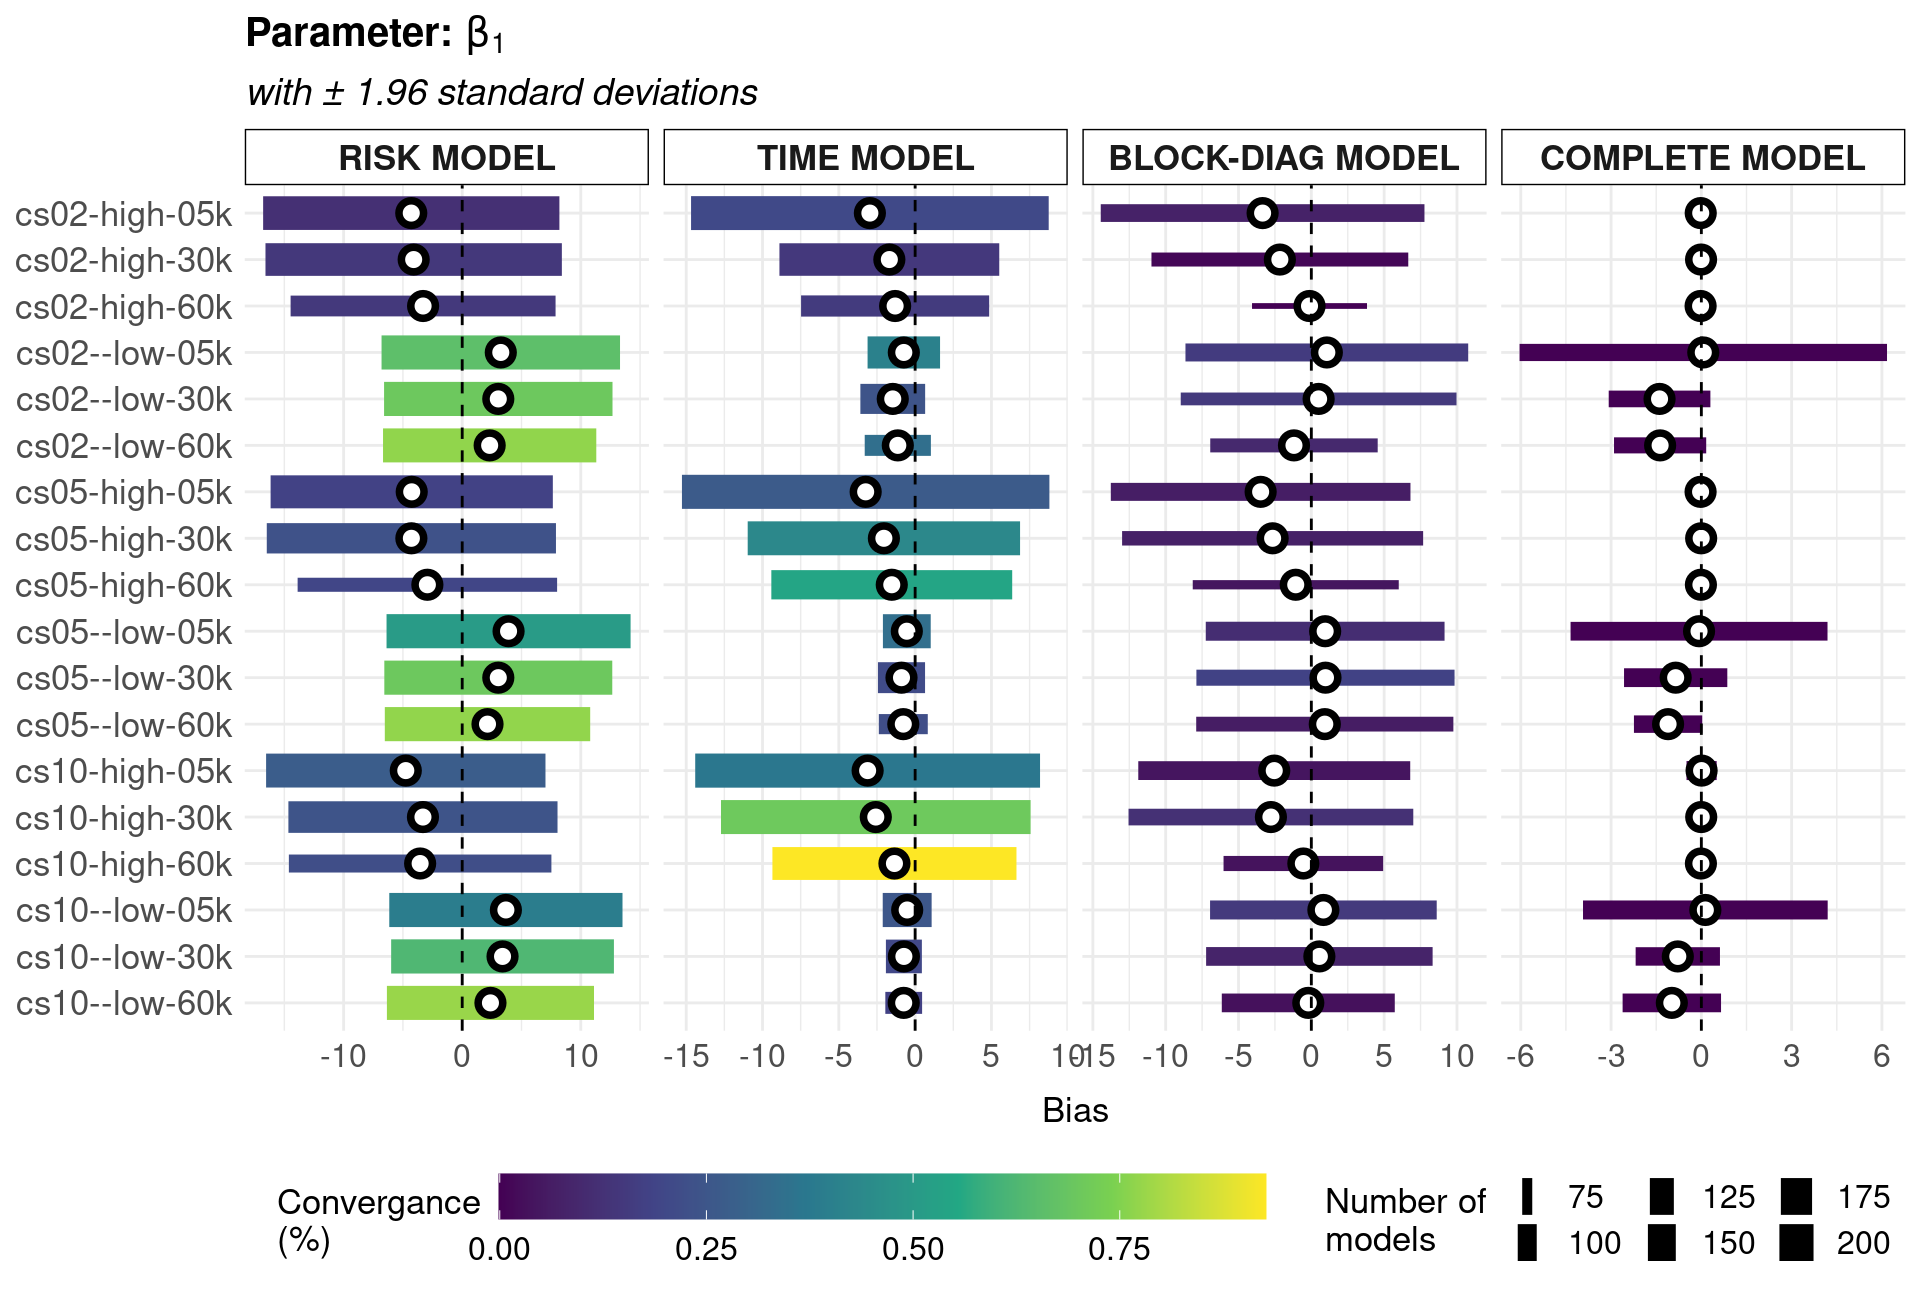
\includegraphics[width=\textwidth]{bias2plotsd-1.png}\\
 \begin{footnotesize}
  SOURCE: The author (2021).
 \end{footnotesize}
 \label{fig:biassdbeta1}
\end{figure}

\begin{figure}[H]
 \setlength{\abovecaptionskip}{.0001pt}
 \caption{PARAMETER \(\beta_{2}\) BIAS WITH \(\pm\) 1.96 STANDARD
         DEVIATIONS}
 \vspace{0.2cm}\centering
 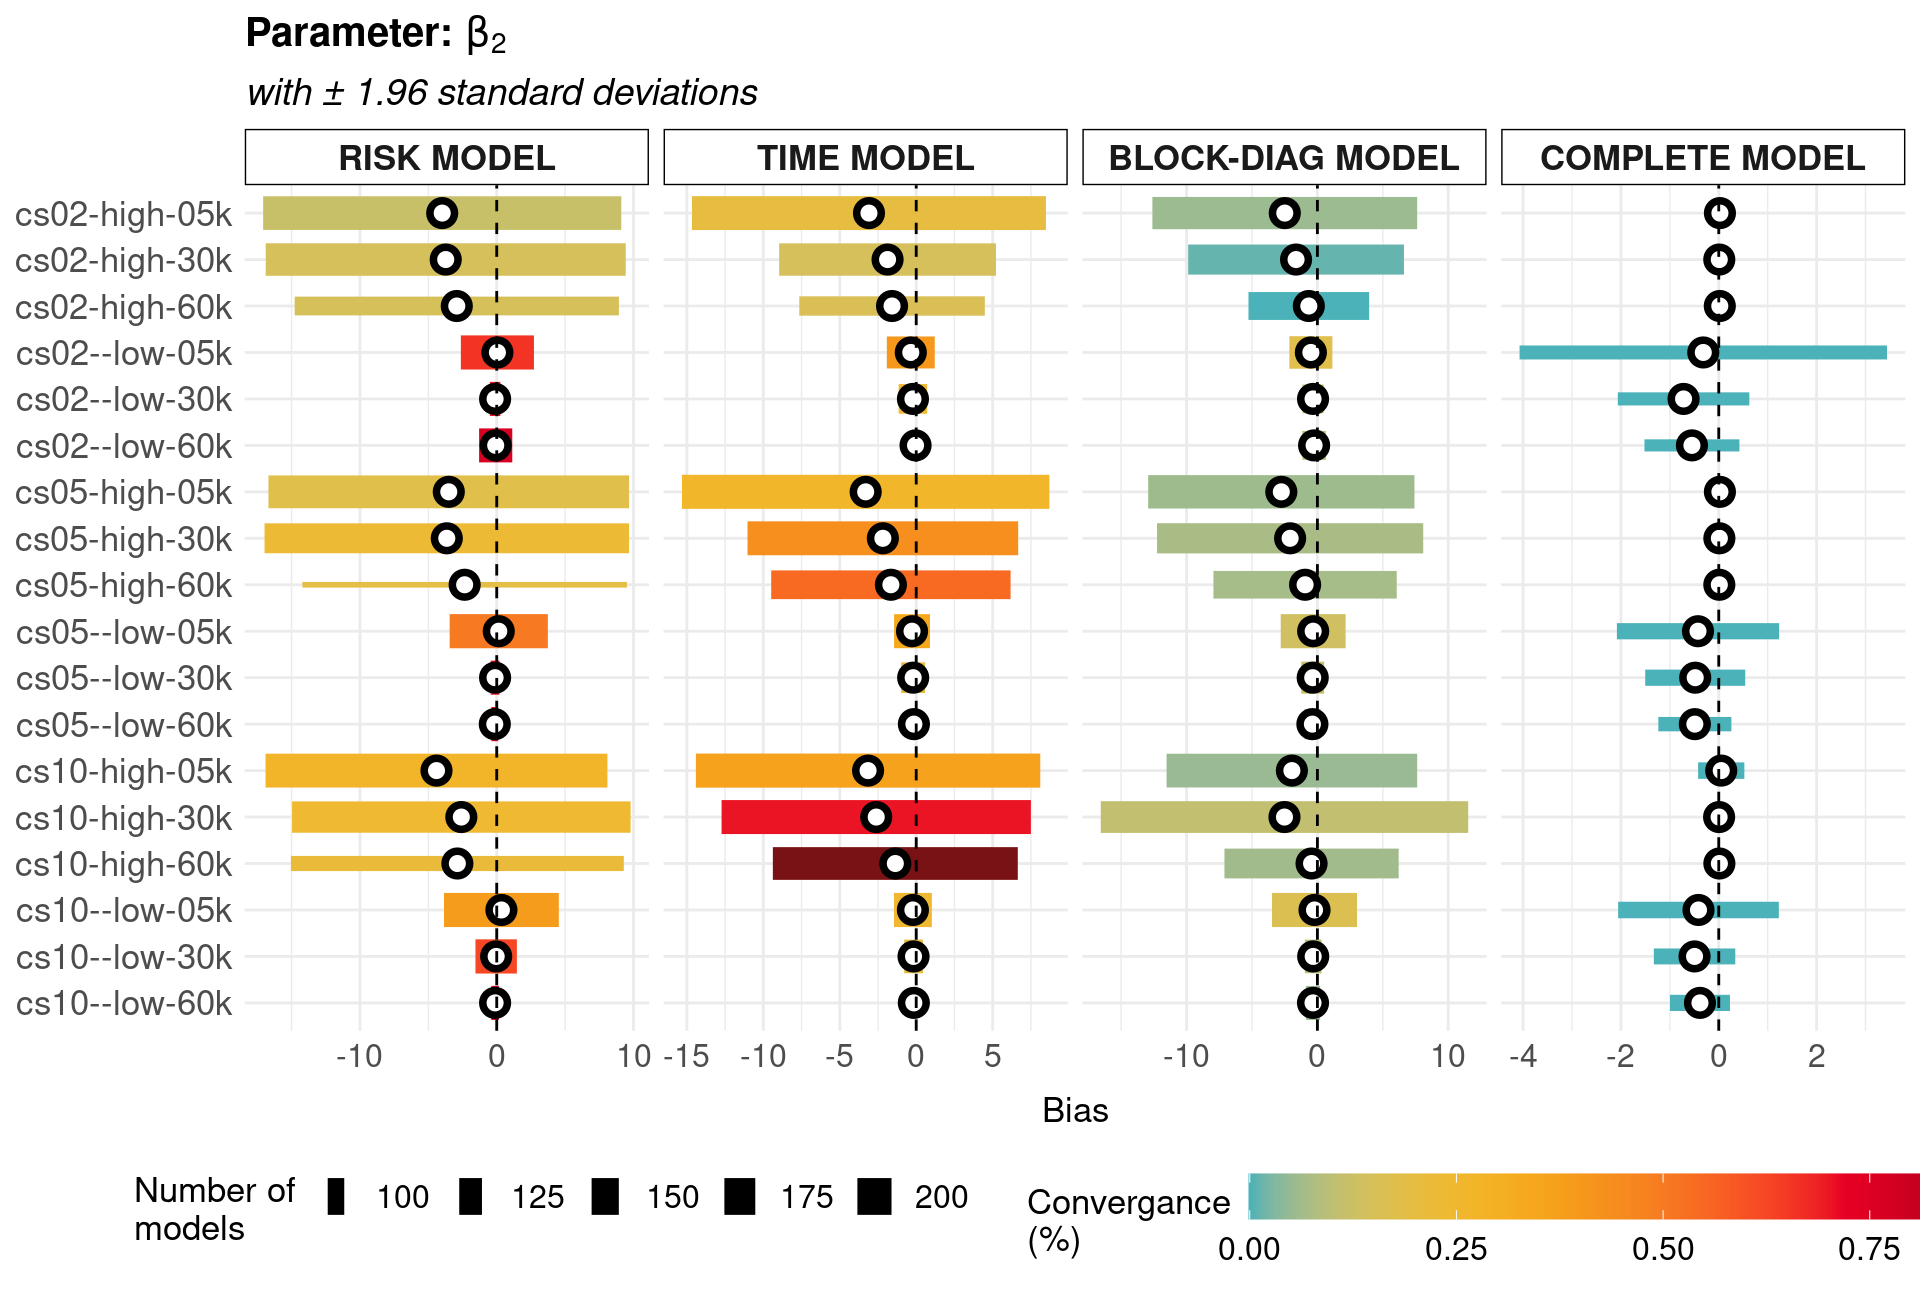
\includegraphics[width=\textwidth]{bias2plotsd-2.png}\\
 \begin{footnotesize}
  SOURCE: The author (2021).
 \end{footnotesize}
 \label{fig:biassdbeta2}
\end{figure}

\begin{figure}[H]
 \setlength{\abovecaptionskip}{.0001pt}
 \caption{PARAMETER \(\gamma_{1}\) BIAS WITH \(\pm\) 1.96 STANDARD
          DEVIATIONS}
 \vspace{0.2cm}\centering
 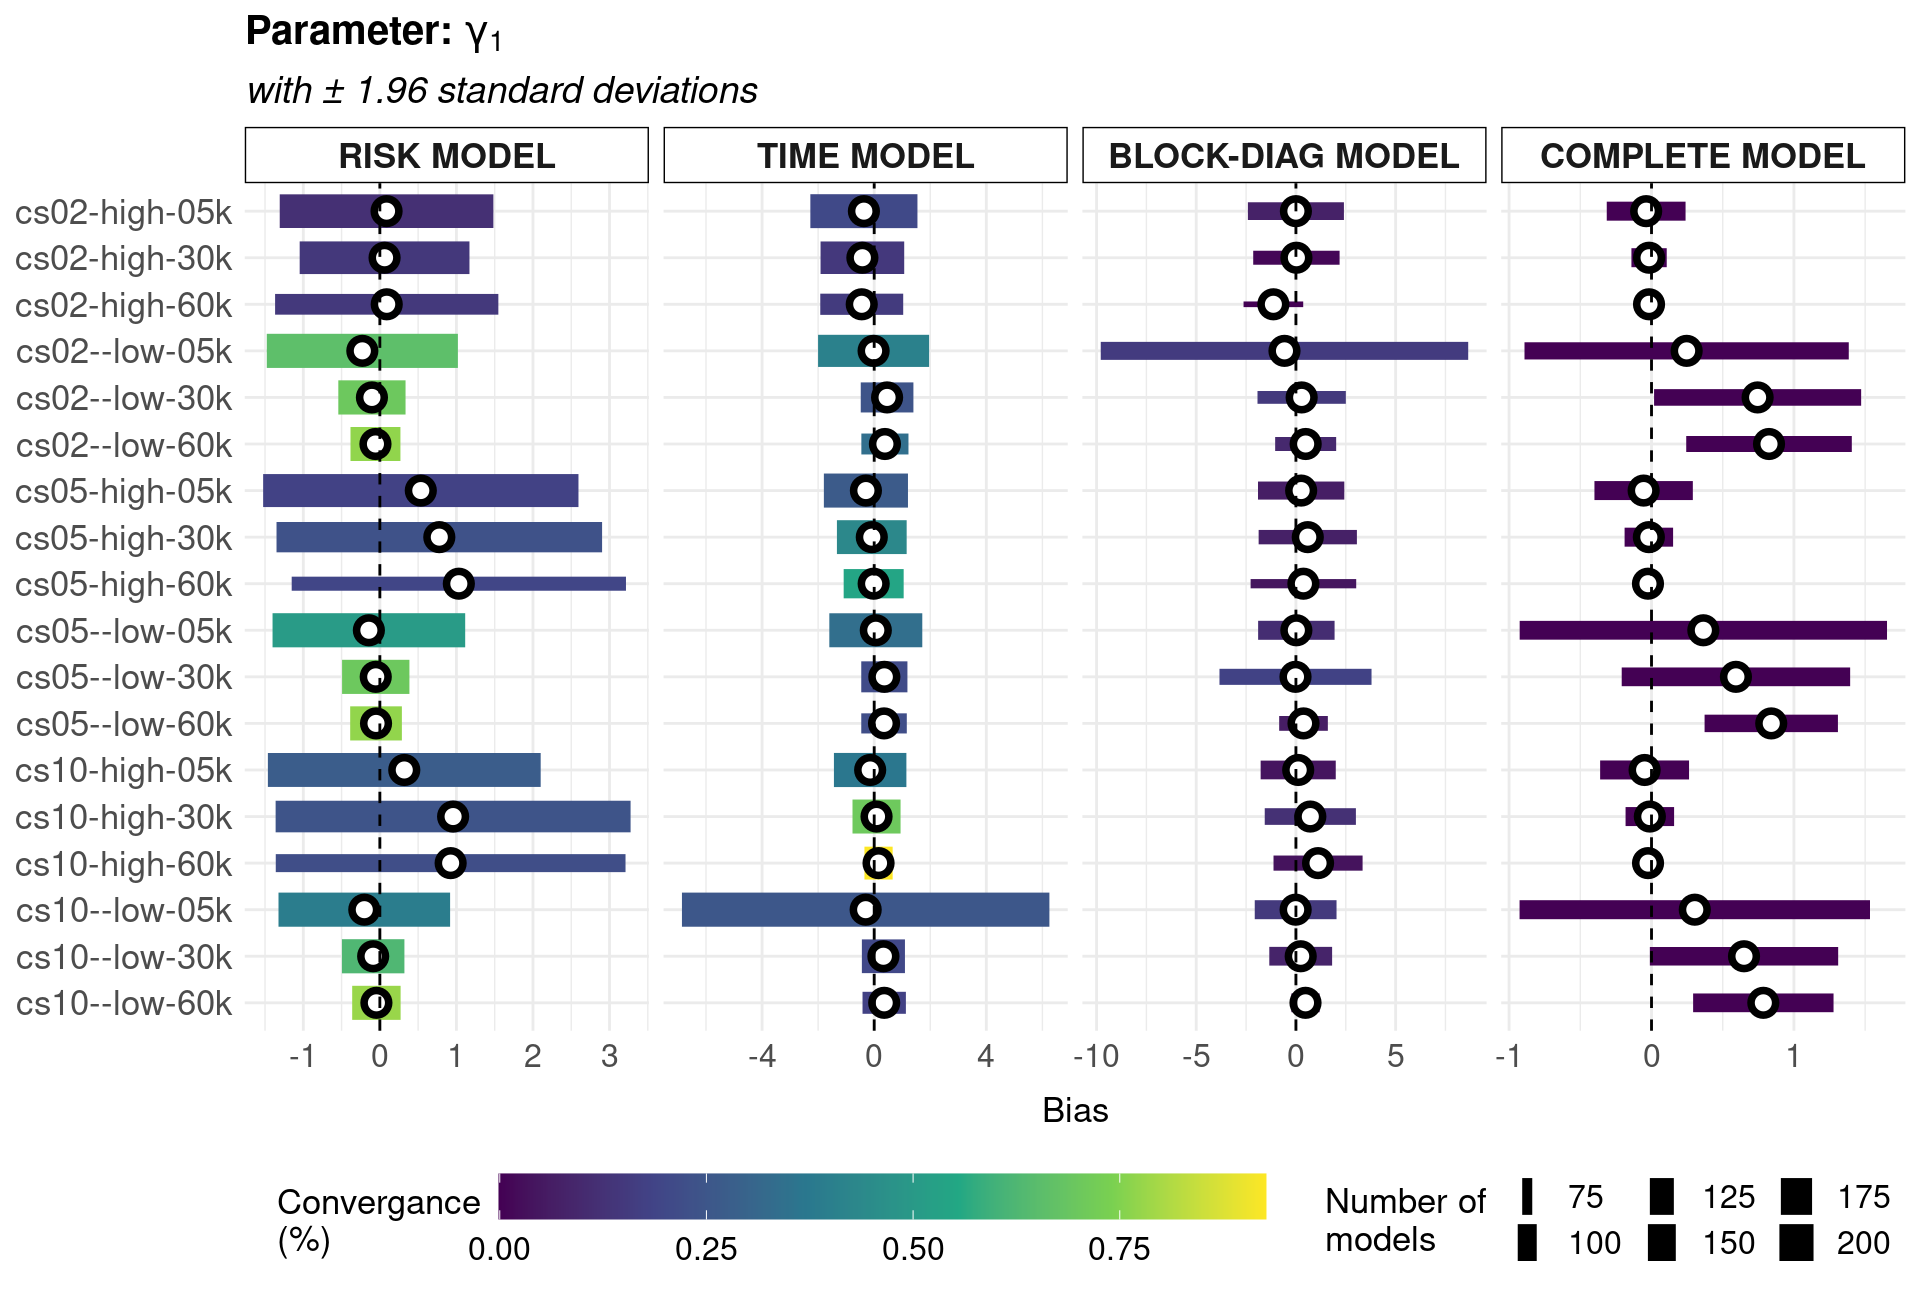
\includegraphics[width=\textwidth]{bias2plotsd-3.png}\\
 \begin{footnotesize}
  SOURCE: The author (2021).
 \end{footnotesize}
 \label{fig:biassdgama1}
\end{figure}

\begin{figure}[H]
 \setlength{\abovecaptionskip}{.0001pt}
 \caption{PARAMETER \(\gamma_{2}\) BIAS WITH \(\pm\) 1.96 STANDARD
          DEVIATIONS}
 \vspace{0.2cm}\centering
 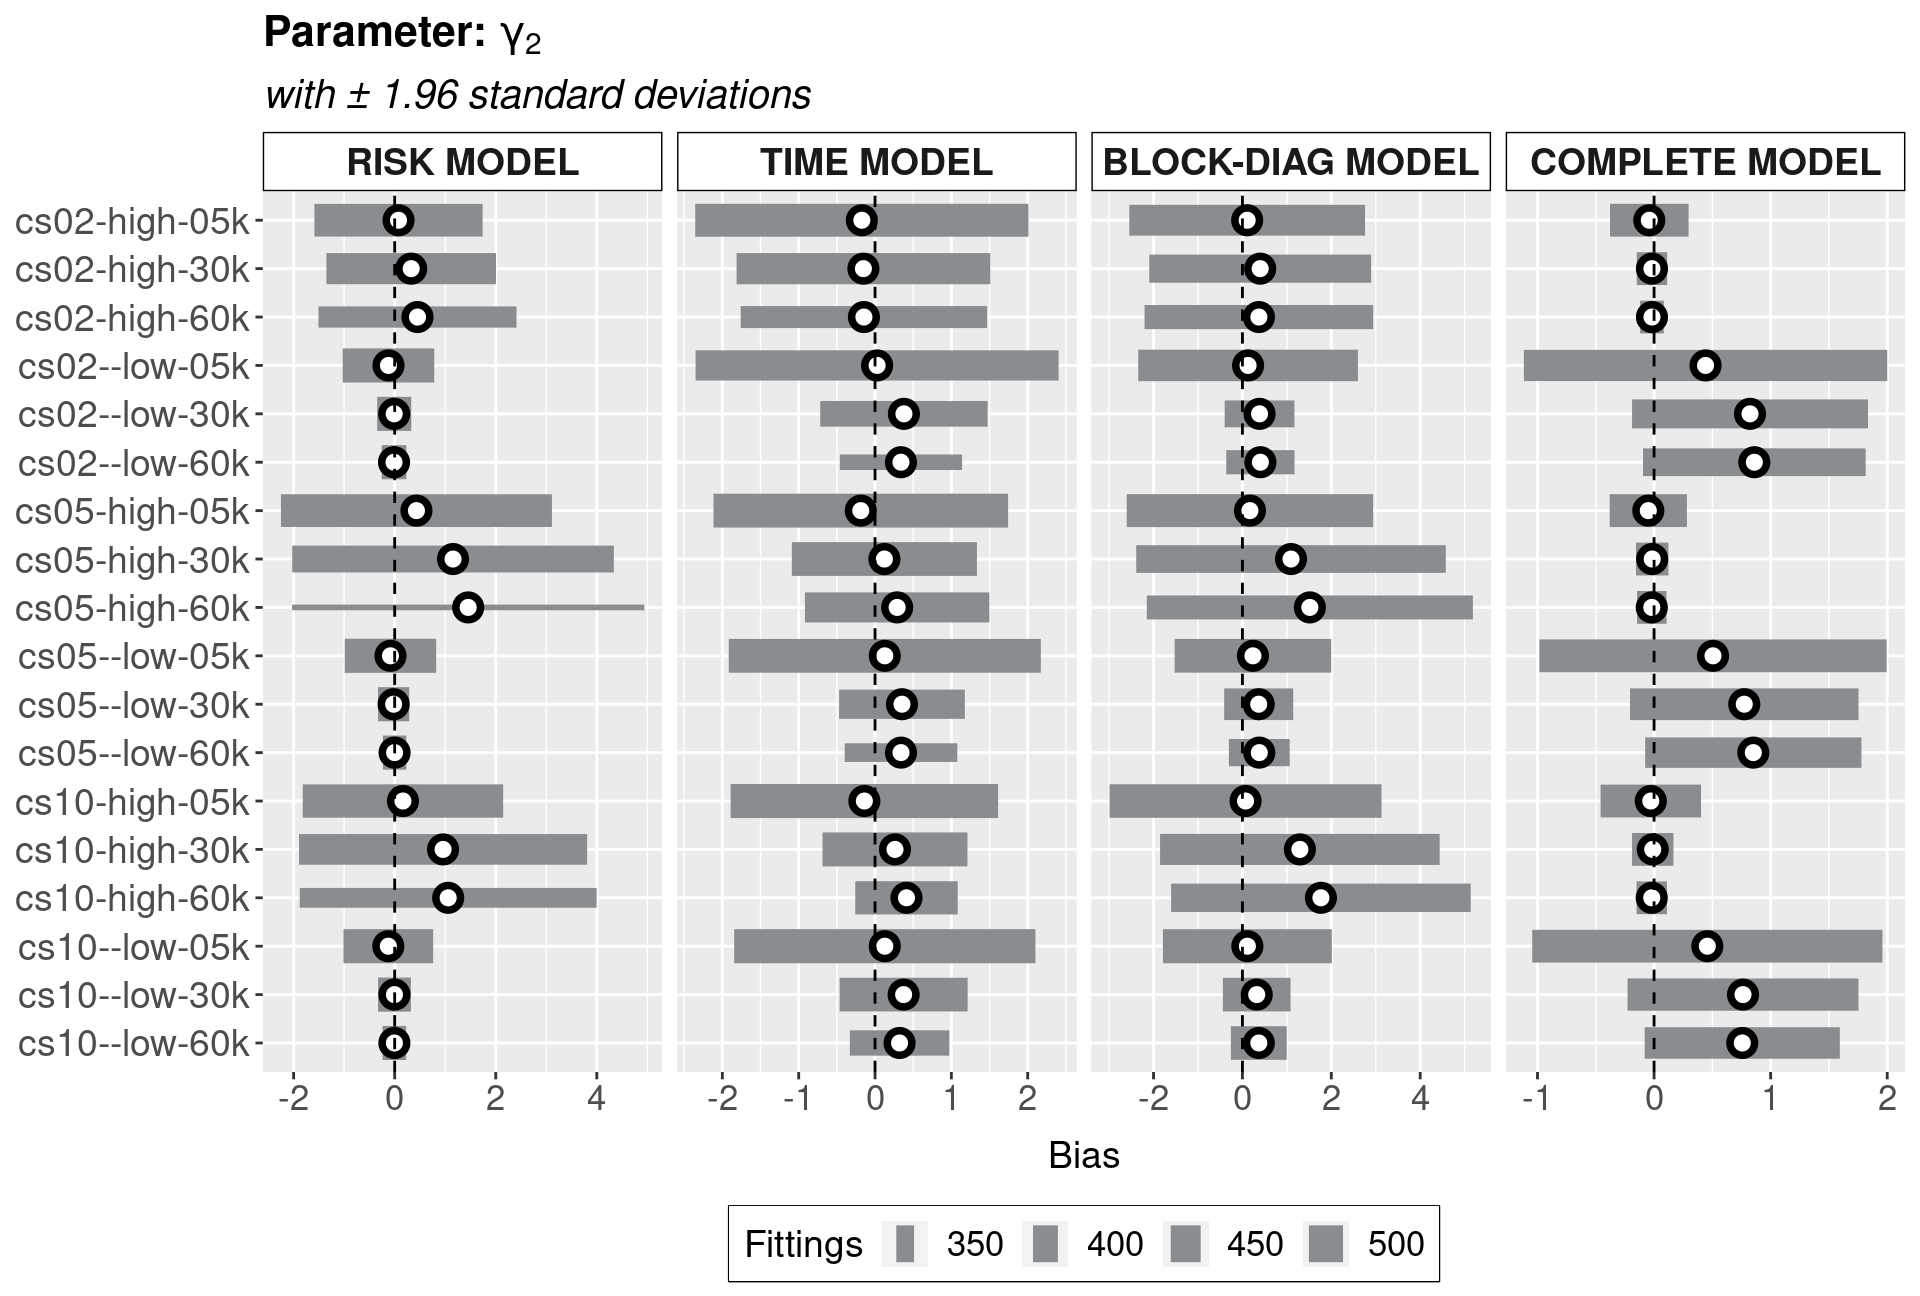
\includegraphics[width=\textwidth]{bias2plotsd-4.png}\\
 \begin{footnotesize}
  SOURCE: The author (2021).
 \end{footnotesize}
 \label{fig:biassdgama2}
\end{figure}

\begin{figure}[H]
 \setlength{\abovecaptionskip}{.0001pt}
 \caption{PARAMETER \(w_{1}\) BIAS WITH \(\pm\) 1.96 STANDARD DEVIATIONS}
 \vspace{0.2cm}\centering
 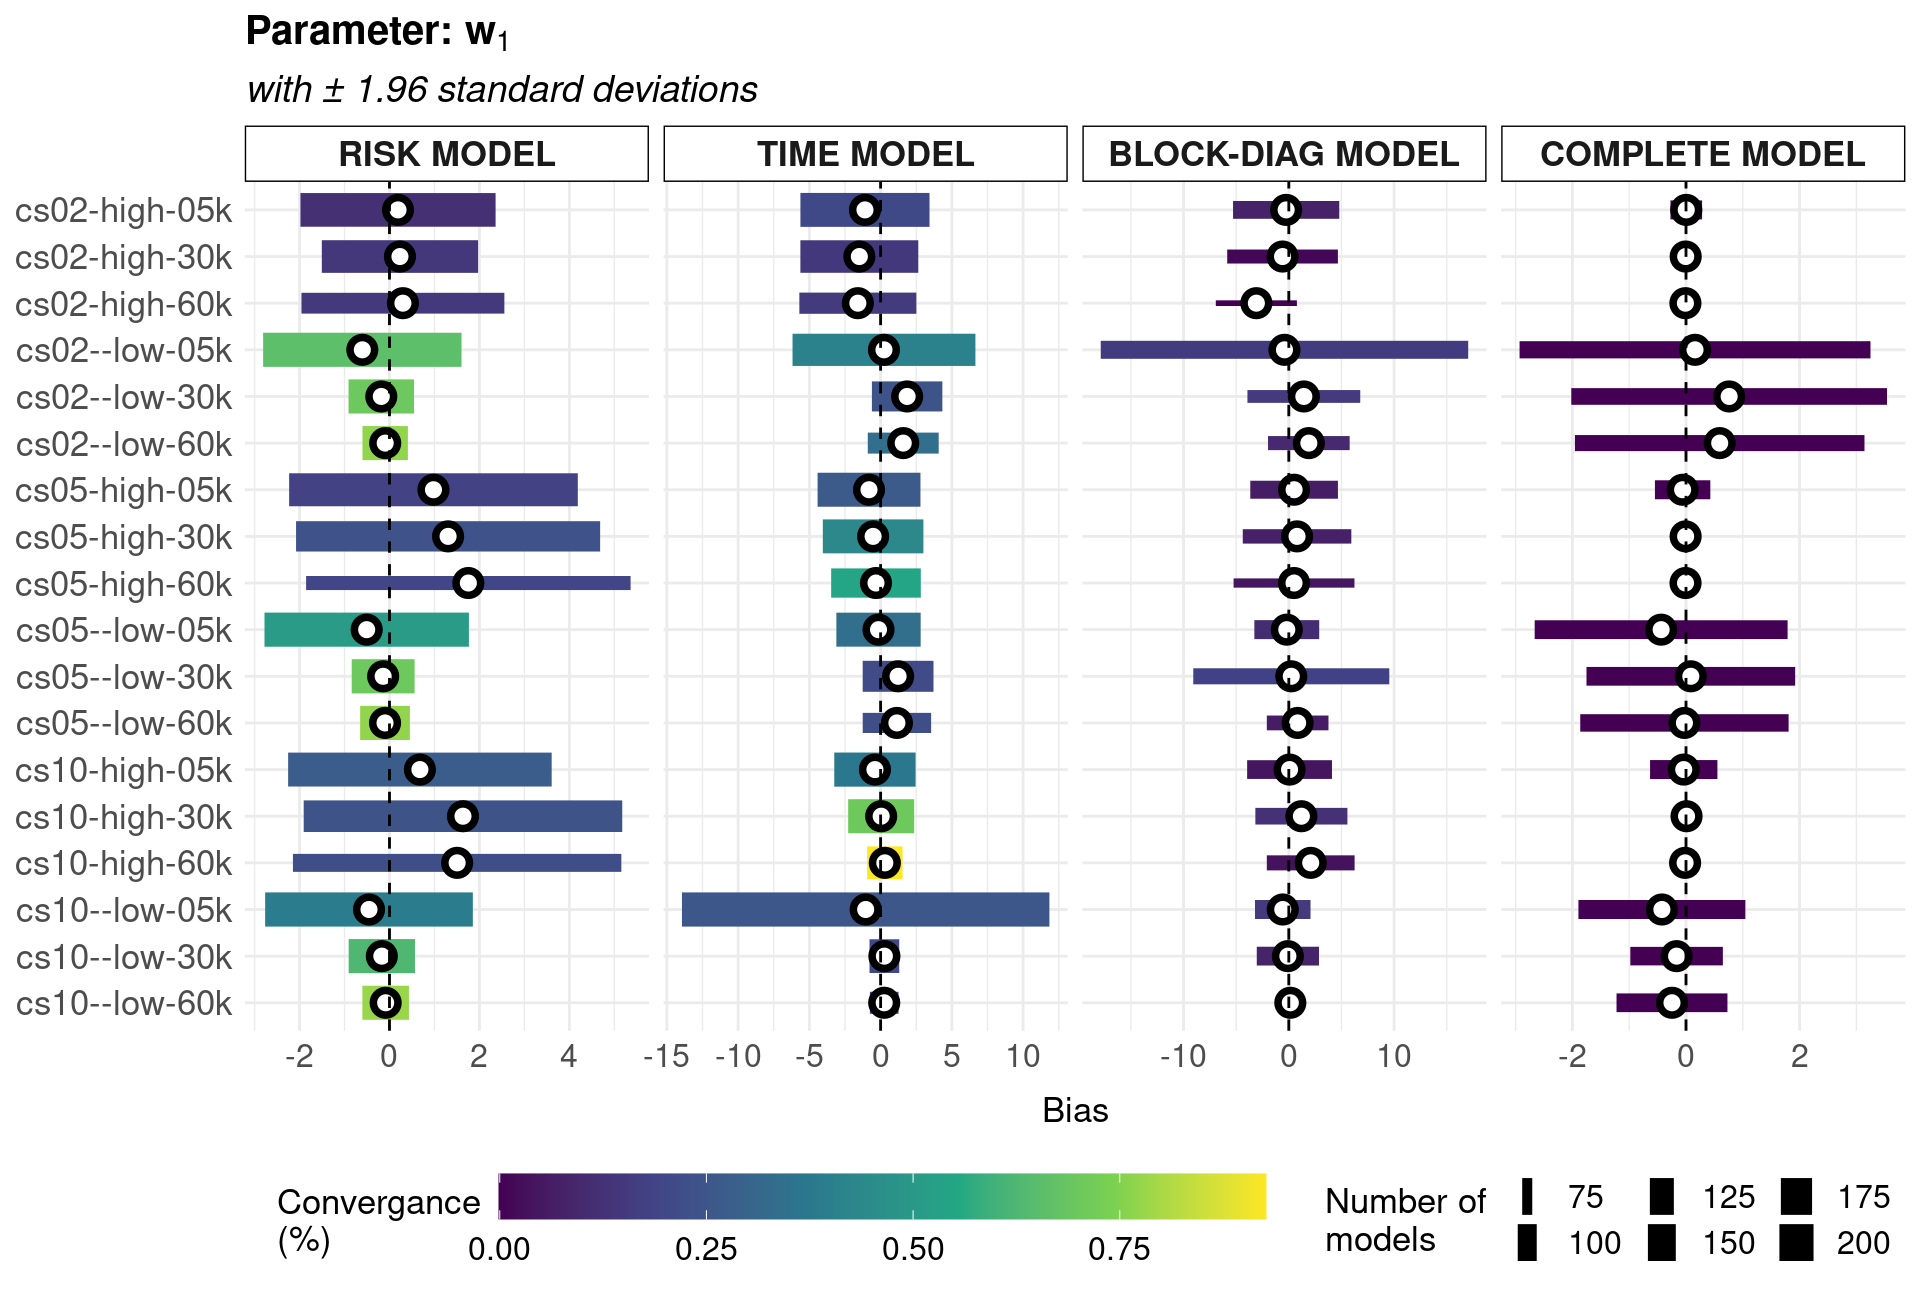
\includegraphics[width=\textwidth]{bias2plotsd-5.png}\\
 \begin{footnotesize}
  SOURCE: The author (2021).
 \end{footnotesize}
 \label{fig:biassdw1}
\end{figure}

\begin{figure}[H]
 \setlength{\abovecaptionskip}{.0001pt}
 \caption{PARAMETER \(w_{2}\) BIAS WITH \(\pm\) 1.96 STANDARD DEVIATIONS}
 \vspace{0.2cm}\centering
 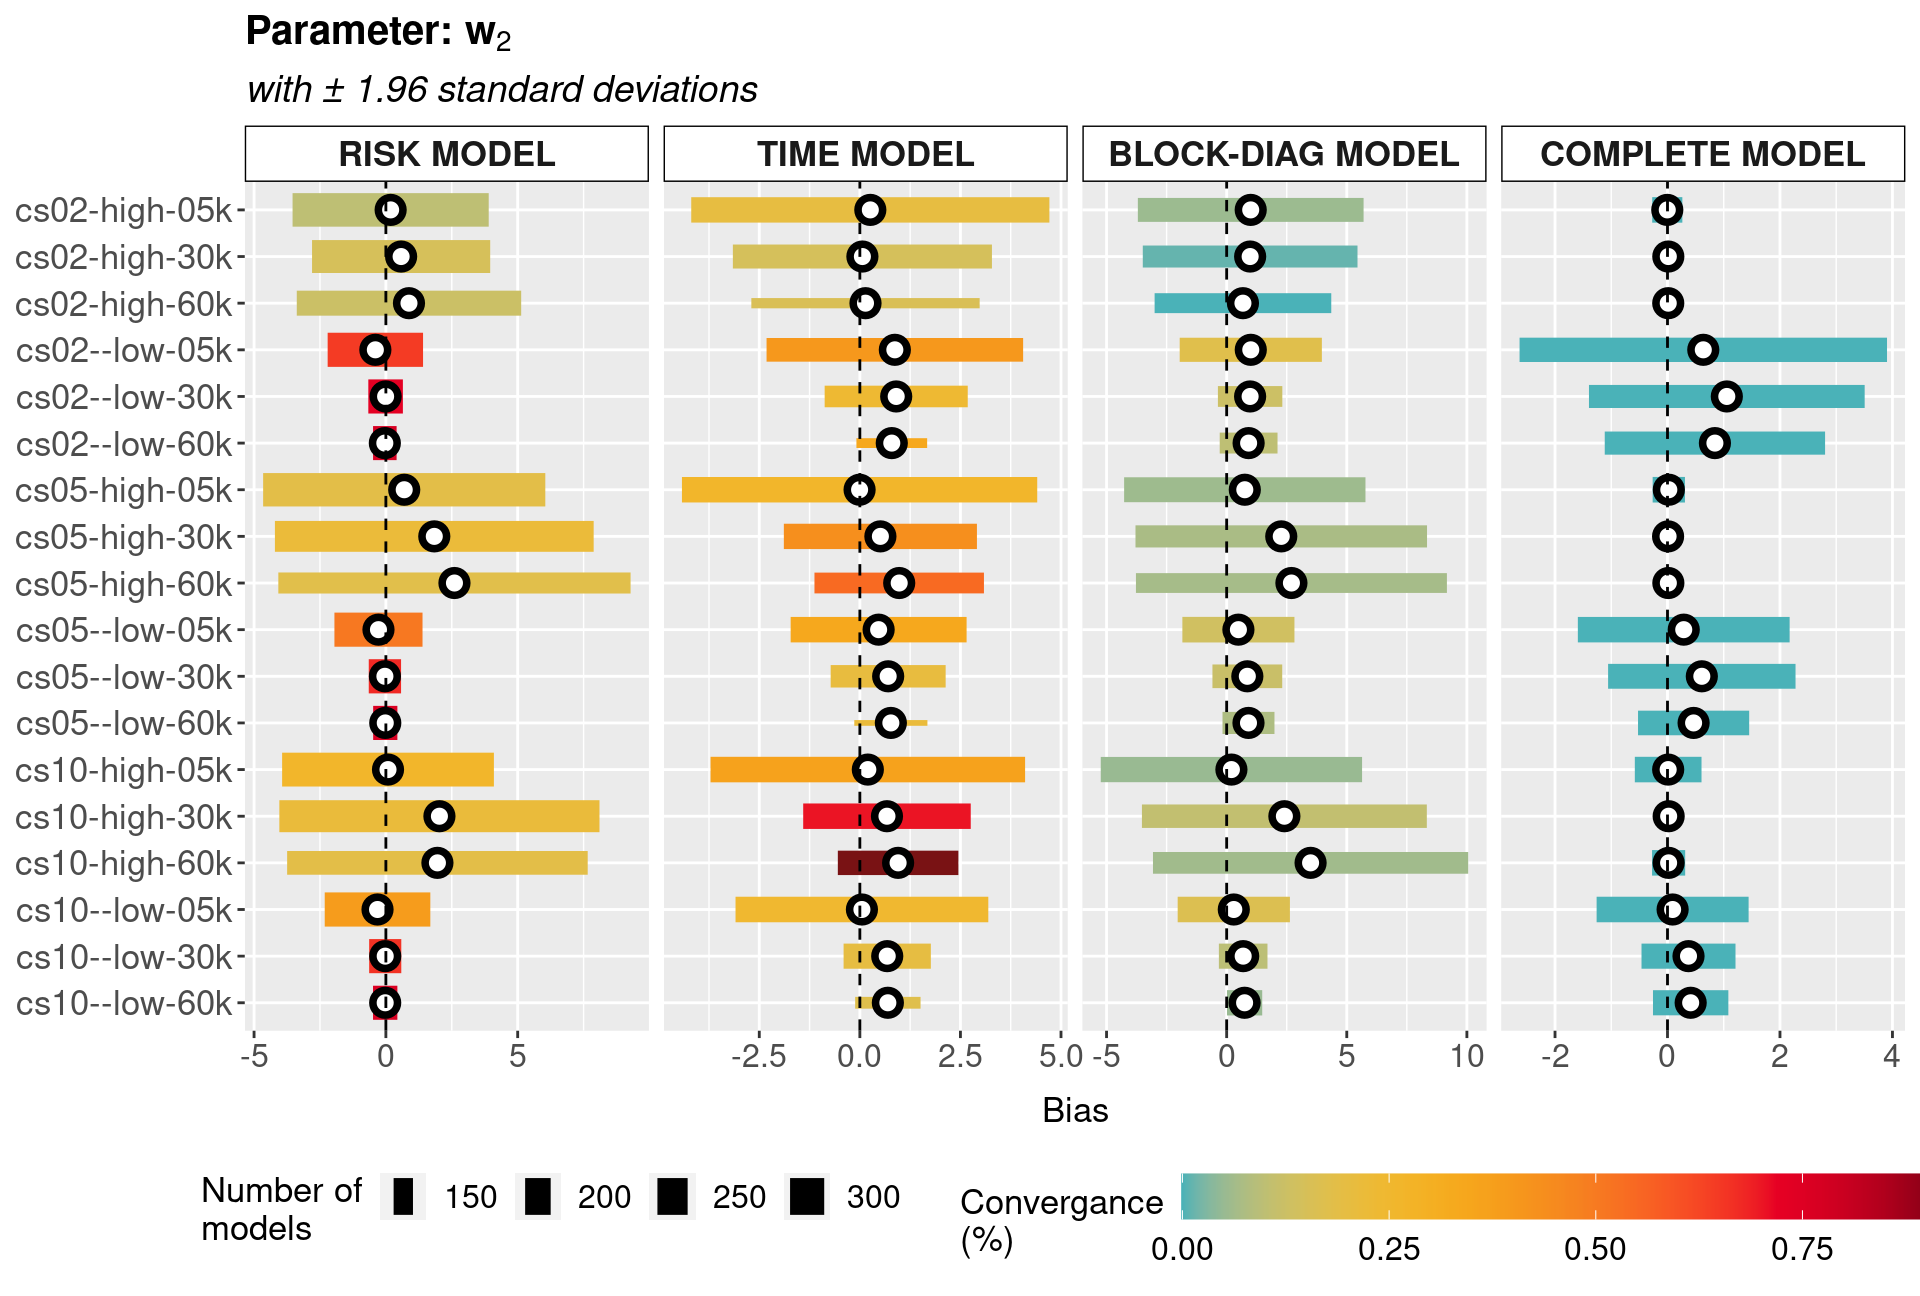
\includegraphics[width=\textwidth]{bias2plotsd-6.png}\\
 \begin{footnotesize}
  SOURCE: The author (2021).
 \end{footnotesize}
 \label{fig:biassdw2}
\end{figure}

\begin{figure}[H]
 \setlength{\abovecaptionskip}{.0001pt}
 \caption{PARAMETER \(\log(\sigma_{1}^{2})\) BIAS WITH \(\pm\) 1.96
          STANDARD DEVIATIONS}
 \vspace{0.2cm}\centering
 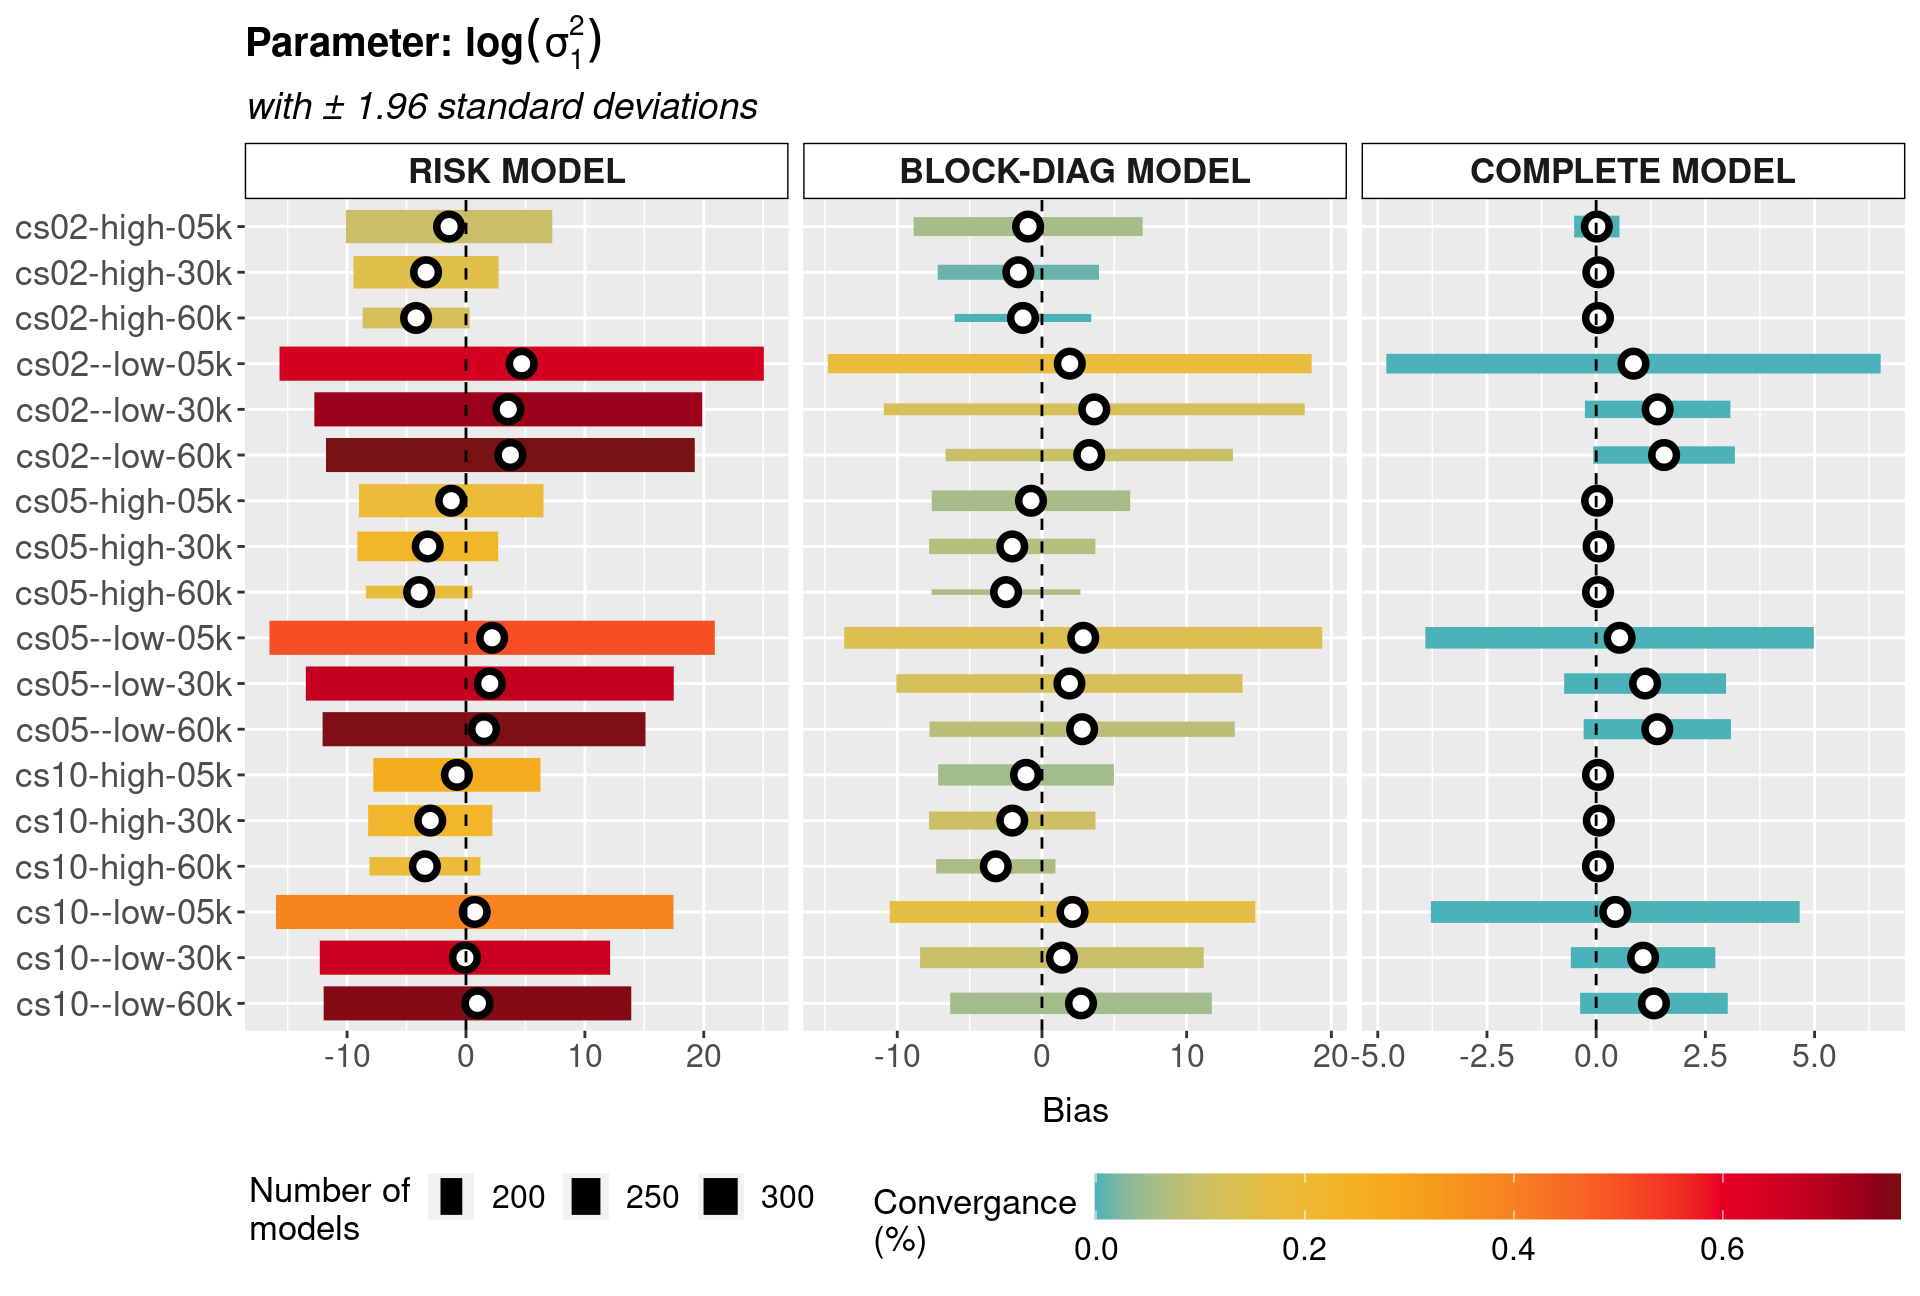
\includegraphics[width=\textwidth]{bias2plotsd-7.png}\\
 \begin{footnotesize}
  SOURCE: The author (2021).
 \end{footnotesize}
 \label{fig:biassdlogs2_1}
\end{figure}

\begin{figure}[H]
 \setlength{\abovecaptionskip}{.0001pt}
 \caption{PARAMETER \(\log(\sigma_{2}^{2})\) BIAS WITH \(\pm\) 1.96
          STANDARD DEVIATIONS}
 \vspace{0.2cm}\centering
 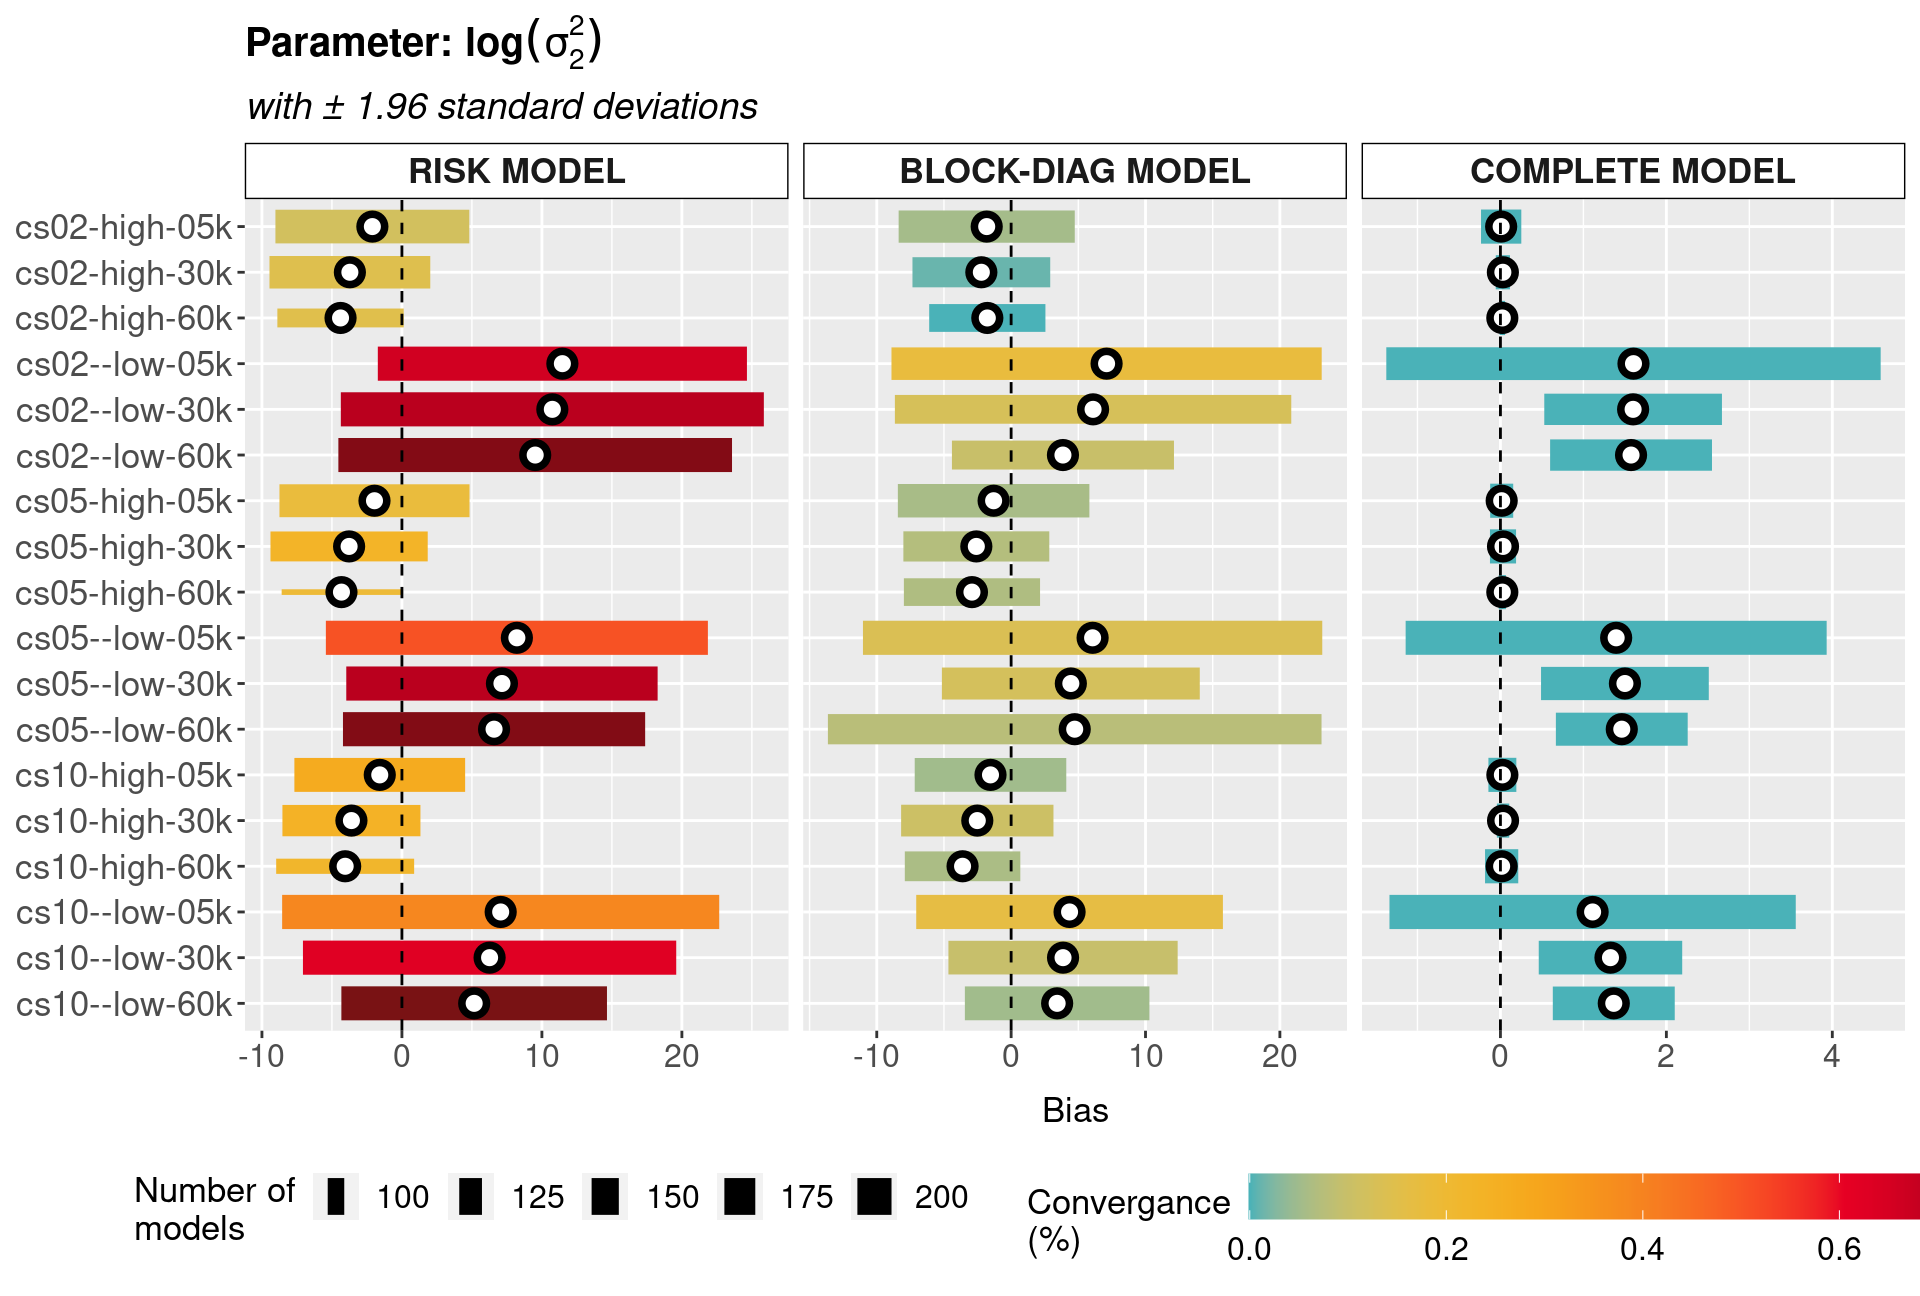
\includegraphics[width=\textwidth]{bias2plotsd-8.png}\\
 \begin{footnotesize}
  SOURCE: The author (2021).
 \end{footnotesize}
 \label{fig:biassdlogs2_2}
\end{figure}

\begin{figure}[H]
 \setlength{\abovecaptionskip}{.0001pt}
 \caption{PARAMETER \(\log(\sigma_{3}^{2})\) BIAS WITH \(\pm\) 1.96
          STANDARD DEVIATIONS}
 \vspace{0.2cm}\centering
 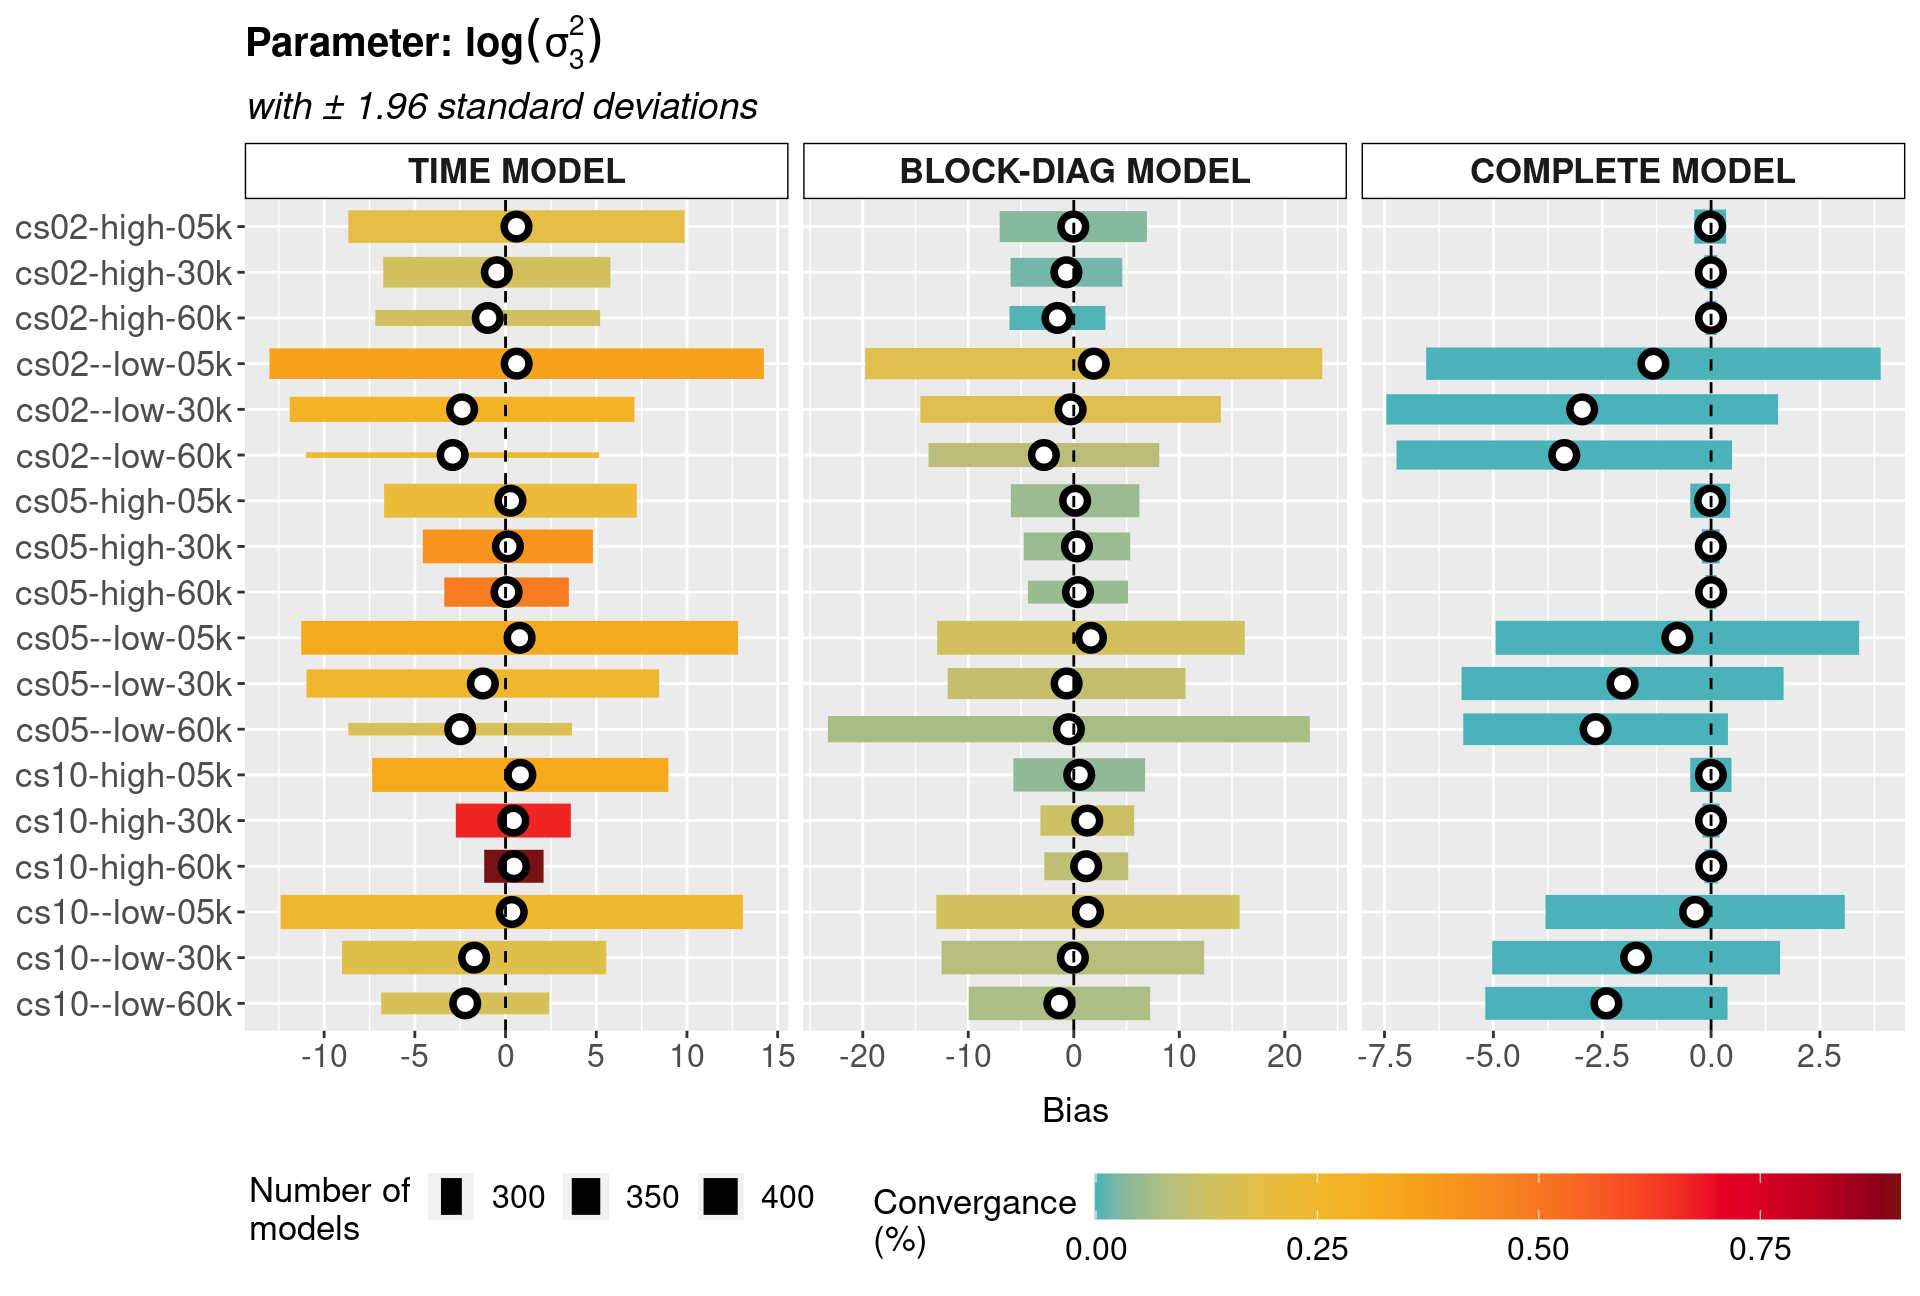
\includegraphics[width=\textwidth]{bias2plotsd-9.png}\\
 \begin{footnotesize}
  SOURCE: The author (2021).
 \end{footnotesize}
 \label{fig:biassdlogs2_3}
\end{figure}

\begin{figure}[H]
 \setlength{\abovecaptionskip}{.0001pt}
 \caption{PARAMETER \(\log(\sigma_{4}^{2})\) BIAS WITH \(\pm\) 1.96
          STANDARD DEVIATIONS}
 \vspace{0.2cm}\centering
 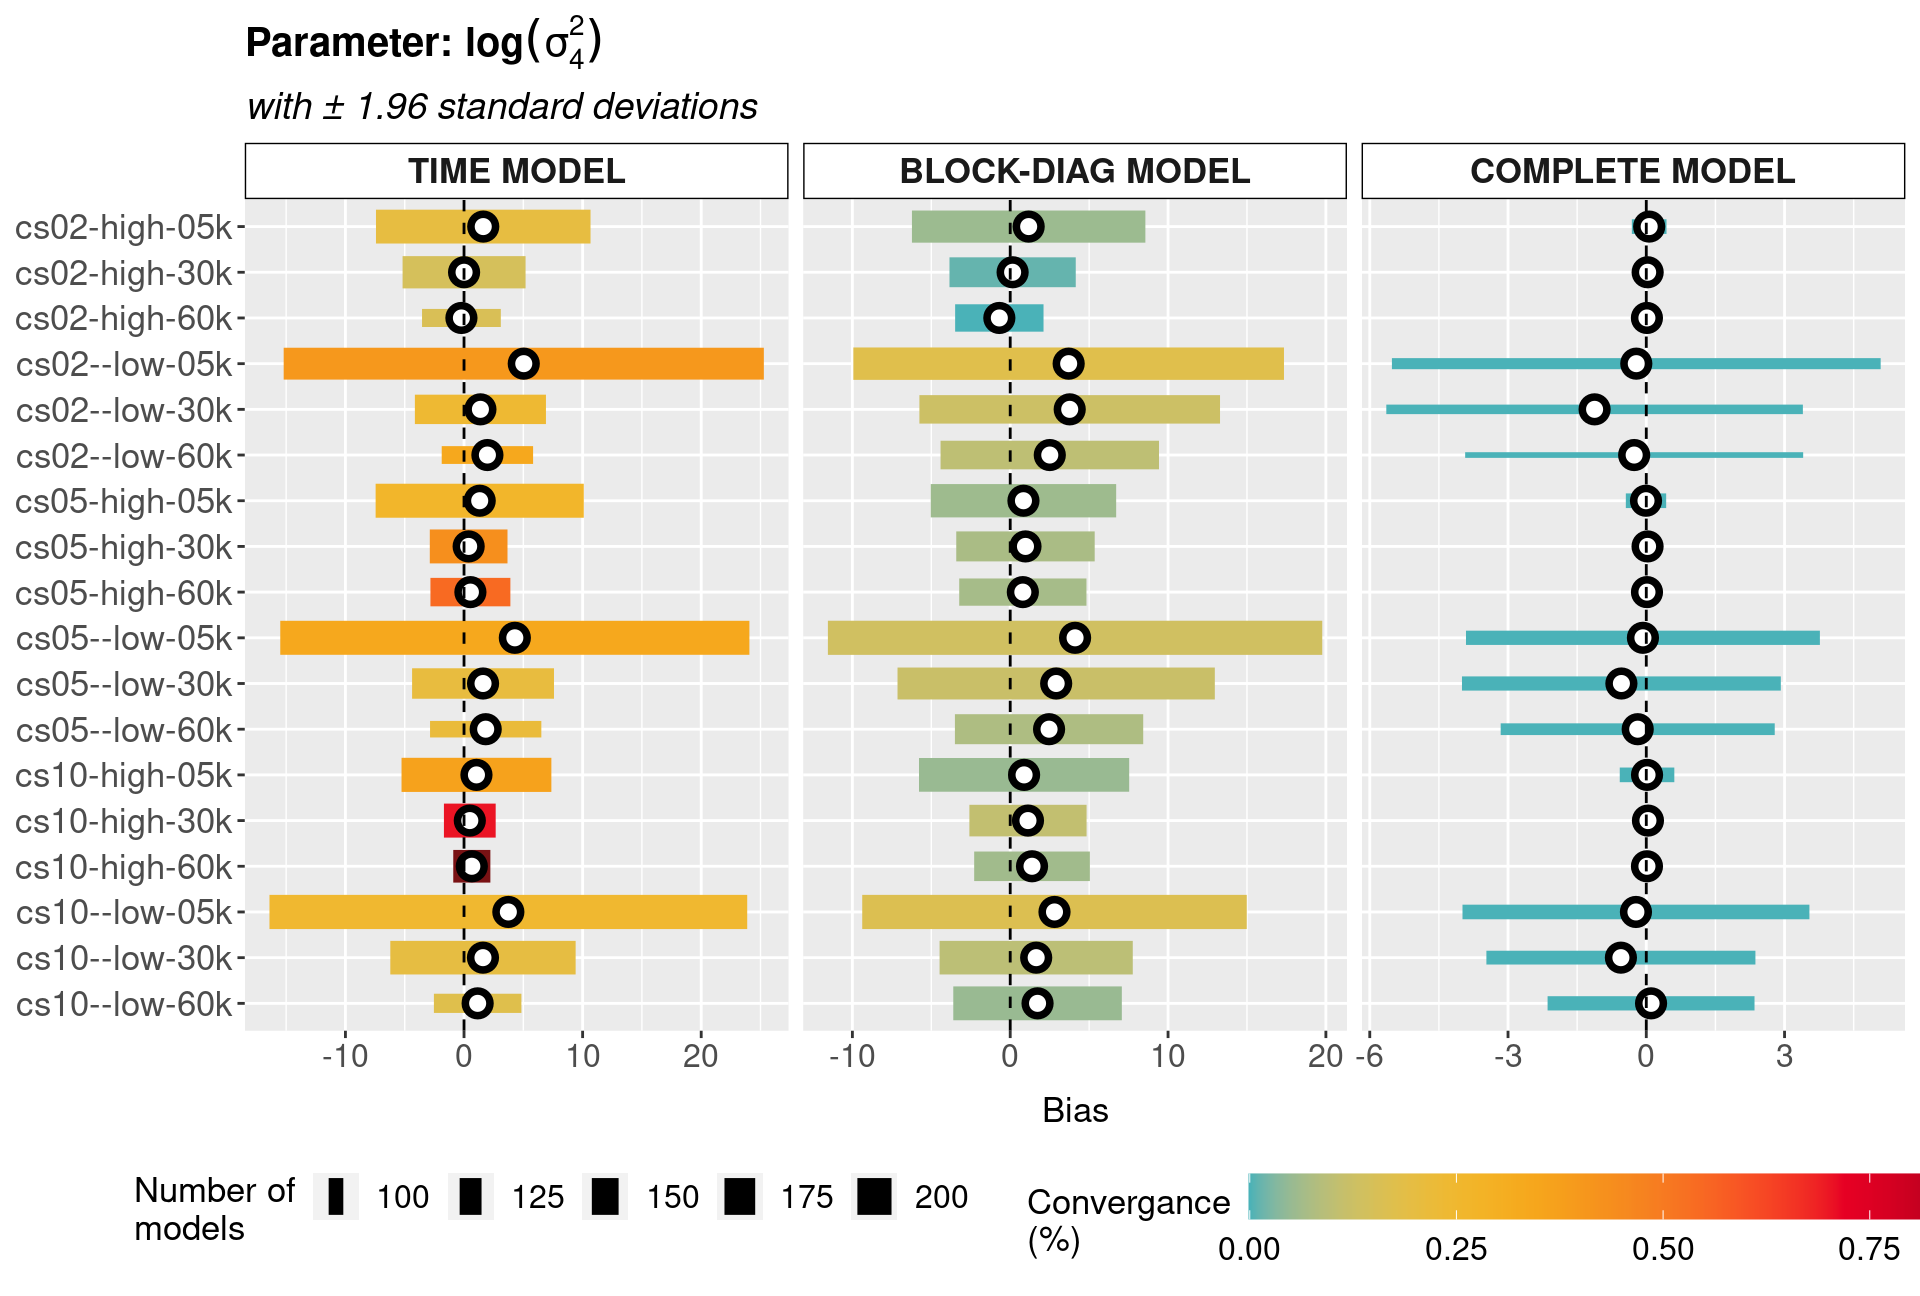
\includegraphics[width=\textwidth]{bias2plotsd-10.png}\\
 \begin{footnotesize}
  SOURCE: The author (2021).
 \end{footnotesize}
 \label{fig:biassdlogs2_4}
\end{figure}

\begin{figure}[H]
 \setlength{\abovecaptionskip}{.0001pt}
 \caption{PARAMETER \(z(\rho_{12})\) BIAS WITH \(\pm\) 1.96 STANDARD
          DEVIATIONS}
 \vspace{0.2cm}\centering
 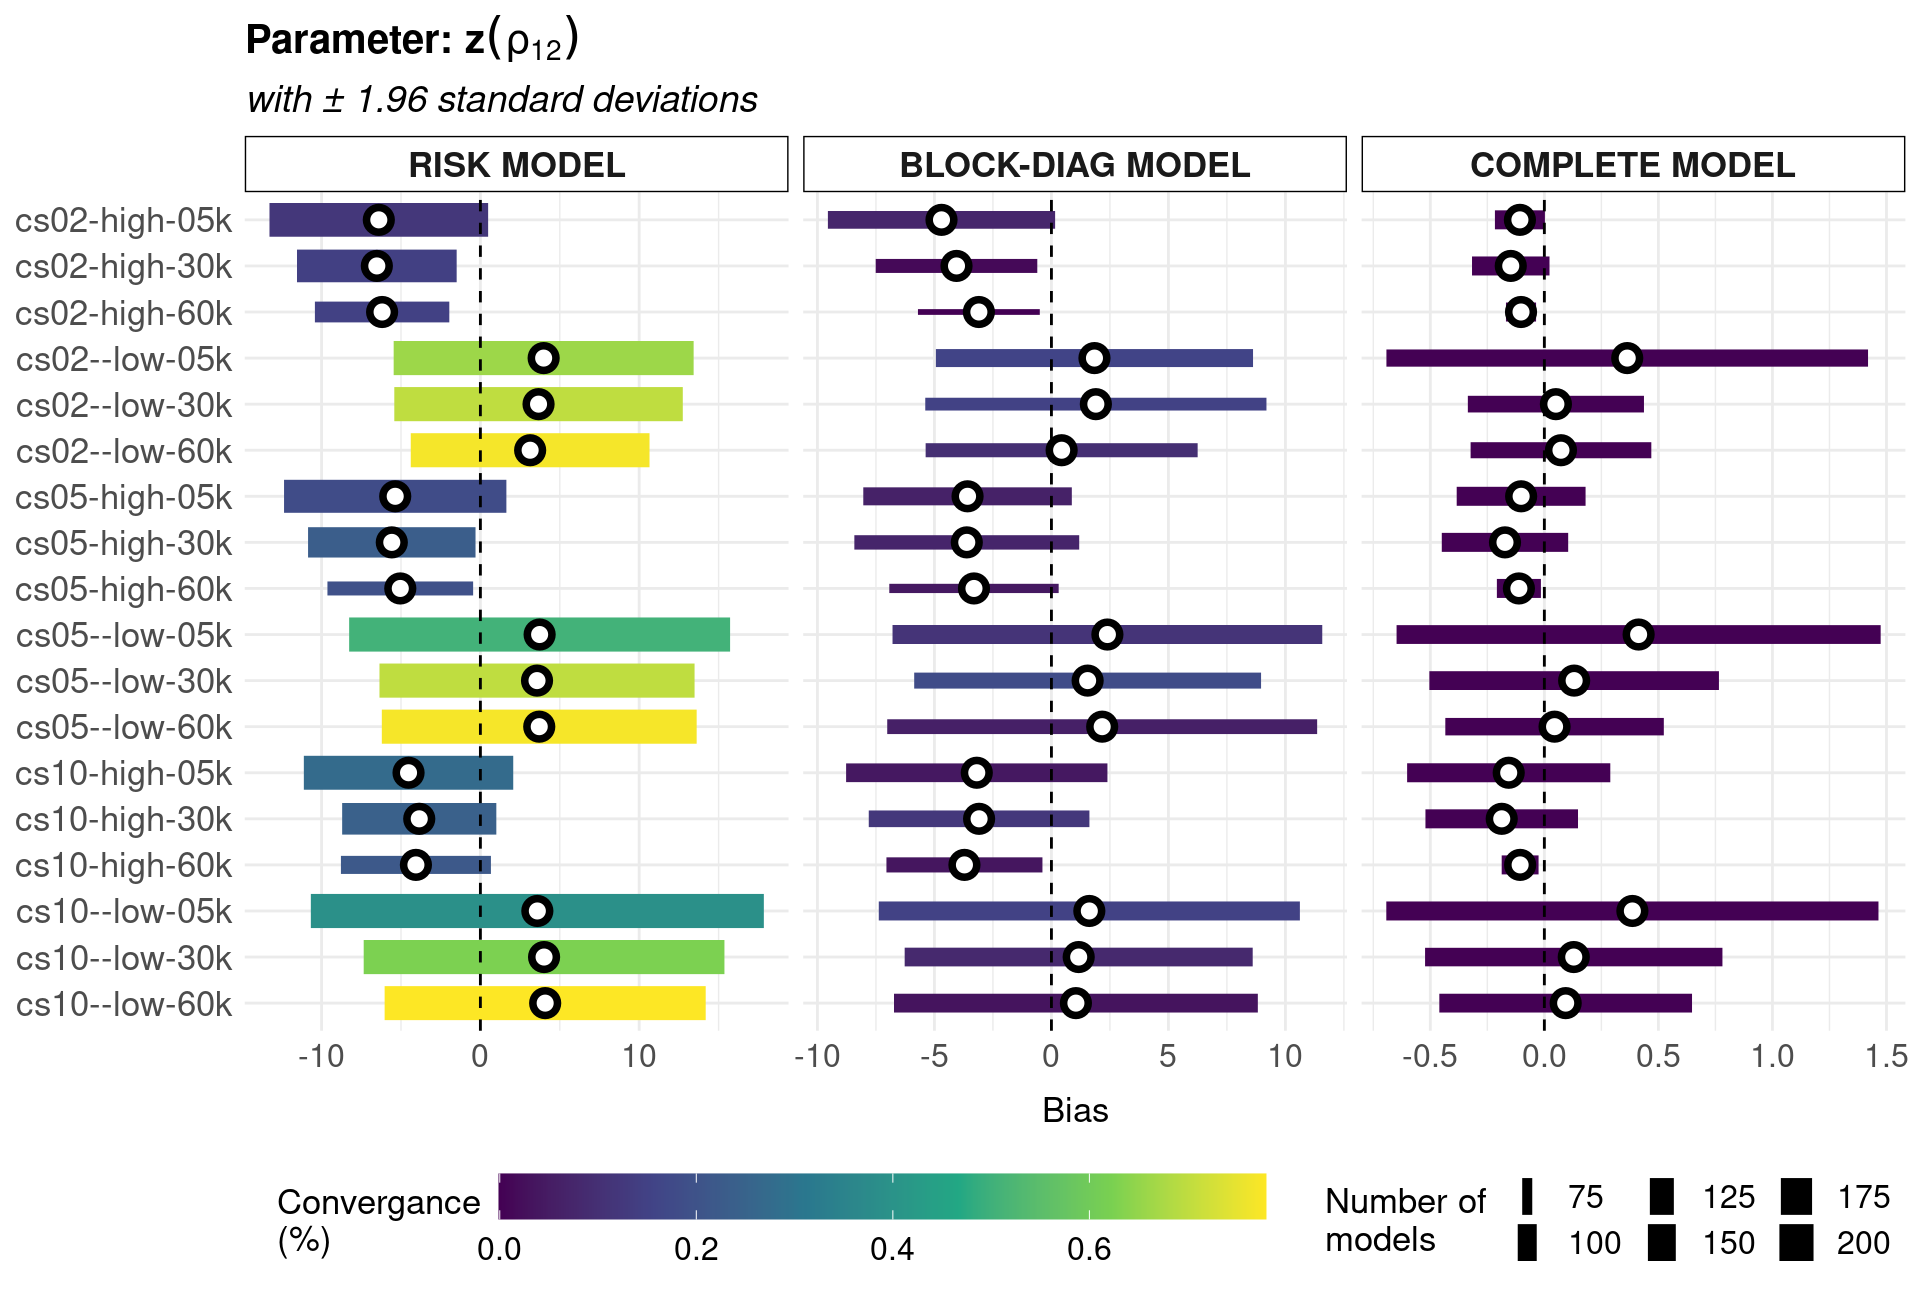
\includegraphics[width=\textwidth]{bias2plotsd-11.png}\\
 \begin{footnotesize}
  SOURCE: The author (2021).
 \end{footnotesize}
 \label{fig:biassdrhoz12}
\end{figure}

\begin{figure}[H]
 \setlength{\abovecaptionskip}{.0001pt}
 \caption{PARAMETER \(z(\rho_{34})\) BIAS WITH \(\pm\) 1.96 STANDARD
          DEVIATIONS}
 \vspace{0.2cm}\centering
 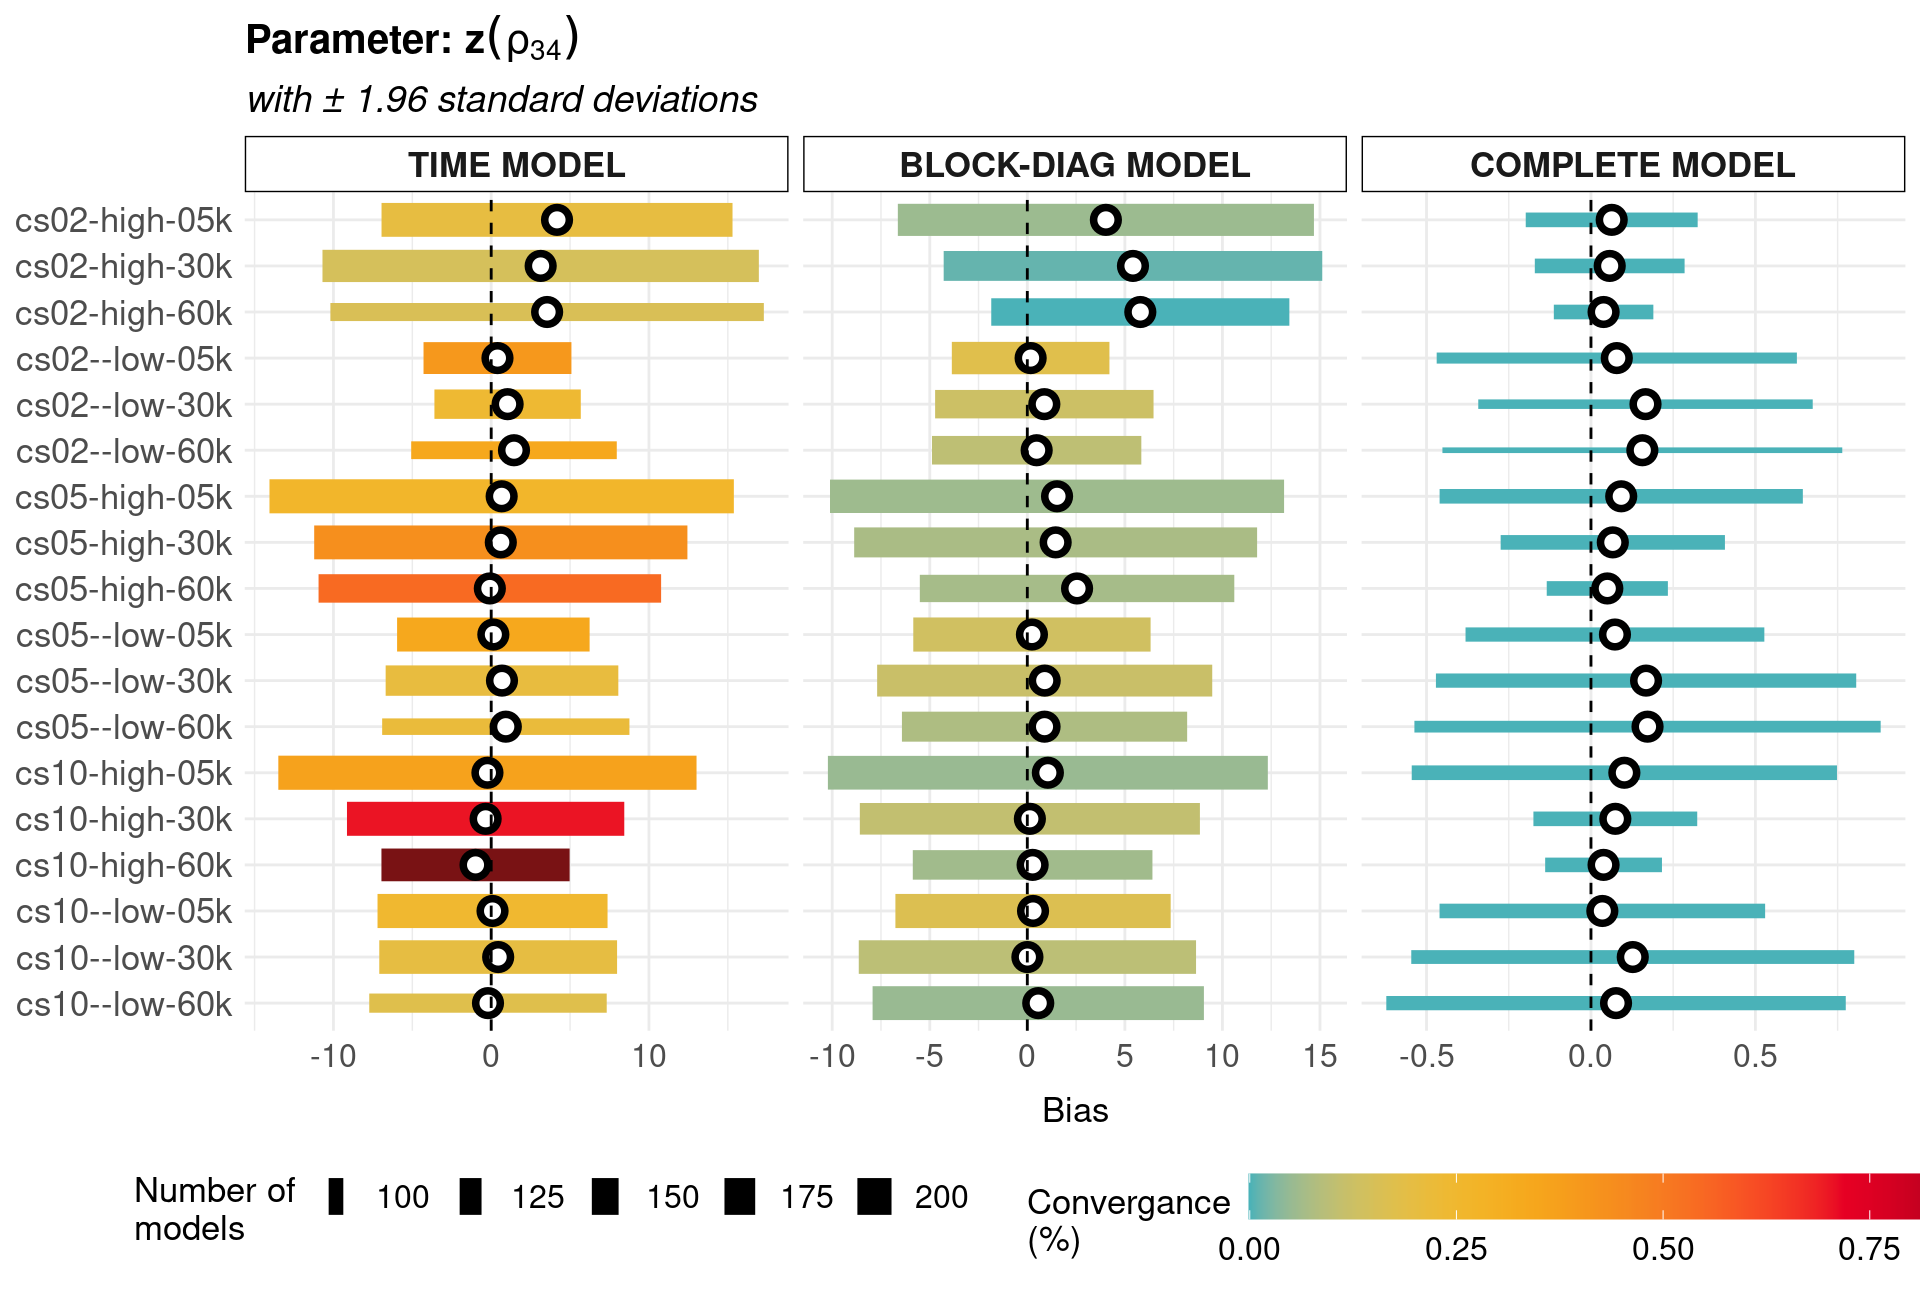
\includegraphics[width=\textwidth]{bias2plotsd-12.png}\\
 \begin{footnotesize}
  SOURCE: The author (2021).
 \end{footnotesize}
 \label{fig:biassdrhoz34}
\end{figure}

\begin{figure}[H]
 \setlength{\abovecaptionskip}{.0001pt}
 \caption{PARAMETERS
          \(\{z(\rho_{13}),~z(\rho_{24}),~z(\rho_{14}),~z(\rho_{23})\}\)
          BIAS WITH \(\pm\) 1.96 STANDARD DEVIATIONS}
 \vspace{0.2cm}\centering
 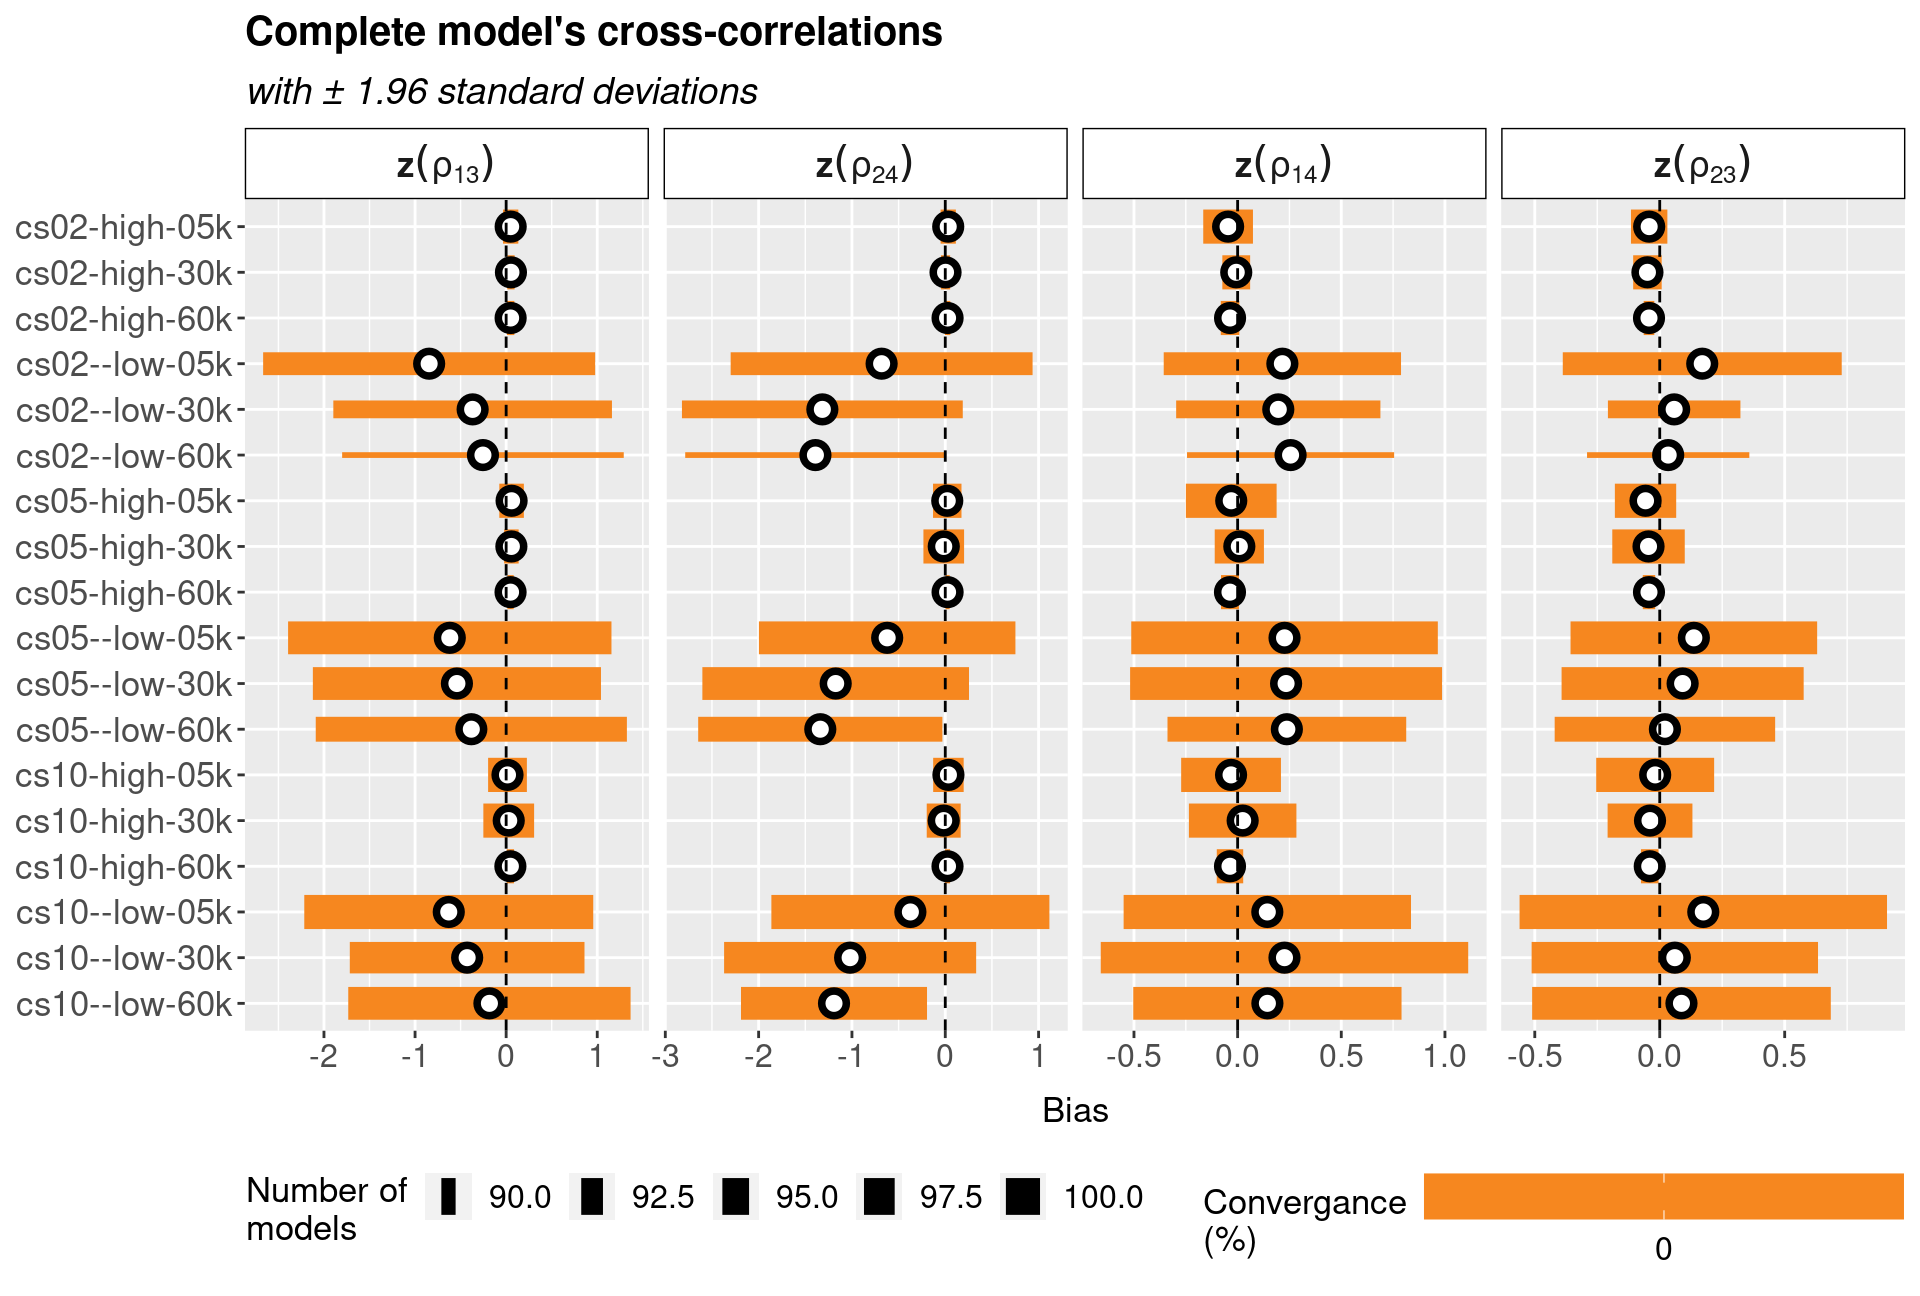
\includegraphics[width=\textwidth]{bias2plotsd-13.png}\\
 \begin{footnotesize}
  SOURCE: The author (2021).
 \end{footnotesize}
 \label{fig:biassdrhoz4}
\end{figure}

In each figure, we have the parameter bias and its uncertainty described
by a Wald-based interval i.e., \(\pm\) 1.96 the bias standard
deviation. This is a good uncertainty representation choice since it is
symmetric and robust to outliers. In the \autoref{cap:appendixD}, we
have the same parameters bias but with the corresponding 2.5 and 97.5\%
quantiles.

The seventy-two scenarios are accommodated. We have up to four blocks of
bars, each block representing a model. In each block we have eighteen
bars, each bar representing the 300 fits in each of the eighteen
scenarios (\(4 \times 18 \times 300 = 21600\)). Each scenario name
consists of a combination of three strings. The cluster size (cs), 2, 5,
and 10; the CIF configuration, high and low; the sample size, 5, 30, and
60 thousand. We have tried to fit a total of 21600 models but not all
converged. Besides that inconvenience, from the ones that converged do
not all converged in the strict sense of the word. To show these two
characteristics respectively, we control the bar widths and colors.

The ideal convergence is the traditional one i.e., based on the
gradient. However, in complicated optimization scenarios as the one we
are here, we can reach a convergence based on a metric different from
the gradient one.

In \texttt{base::nlmimb()} \texttt{R}'s \texttt{PORT} implementation,
when the default gradient-based convergence is reached we get a 0
message. When the optimization converges but not gradient-based, we get
a 1 message. Looking at the technical report of \citeonline{PORTreport},
we see that this convergence style means that the last algorithm iterate
\(x\) appears to be at a certain scaled distance of the locally optimal
point \(x^{\ast}\). This scaled distance, \(p(x, x^{\ast})\), is defined
by
\[
 p(x, y) =
 \underset{1~\leq i~\leq~p}{\text{max}}
 \left\{d_{i}, |x_{i} - y_{i}|\right\}
 \Big/
 \underset{1~\leq j~\leq~p}{\text{max}}
 \left\{d_{j}, |x_{j}| + |y_{j}|\right\},
\]
where \(d\) is a certain scale vector. In all figures, the considered
convergence percentage is from the gradient-based one.

Something specific can be said about each parameter but let us keep the
focus on the general remarks. Starting from the fixed-effect parameters
(\autoref{fig:biassdbeta1}, \autoref{fig:biassdbeta2},
\autoref{fig:biassdgama1}, \autoref{fig:biassdgama2},
\autoref{fig:biassdw1}, \autoref{fig:biassdw2}), we have some very nice
results that already show a strong inclination to the complete model's
choice.

With a simpler latent structure i.e., a latent structure only in one
level (risk and time models), the low CIF scenarios present a much
smaller bias-variance. In general, the mean-bias is small (good), but
the variances are high. When we have a latent structure on both levels
but assuming the cross-correlations as zero (block-diag model), the
results get a little bit better. Nevertheless, when we assume a non-zero
cross-correlation structure (complete model) basically everything
changes. The mean biases get closer to zero, the standard deviations
decrease 50\% or more, and mainly, now the high CIF scenarios are the
ones with a much smaller bias-variance. All this is accomplished through
the consideration of the cross-correlations.

In the \textit{simpler} models is hard to see some significant
difference between the cluster and sample sizes. In the complete model,
the difference is clear: as we increase the cluster and the sample size
the bias-variance decrease. The mean-bias is basically always the
same. In the risk and block-diag models is hard to point-out a scenario
as the best or worst. For the time model, in two parameters, with the
scenario of cluster size ten; low CiF; and five thousand data points, we
get a much bigger standard deviation.

With the log-variances (\autoref{fig:biassdlogs2_1},
\autoref{fig:biassdlogs2_2}, \autoref{fig:biassdlogs2_3},
\autoref{fig:biassdlogs2_4}), we have instead a similar behavior through
the models. For all models, the high CIF scenarios are the ones with a
smaller mean and bias-variance. From the risk/time model to the
block-diag model, we do not see a significant improvement in terms of
bias reduction. Such improvement, however, is clear when we look at the
complete model. Again, the magick of considering the cross-correlations.

The same said about the log-variances, can be applied to the risk
correlation (\autoref{fig:biassdrhoz12}) with one addendum: the bias
reduction is even bigger. With the time correlation
(\autoref{fig:biassdrhoz34}), we get the same behavior observed with the
fixed-effect parameters i.e., in the simpler models, the smaller biases
are observed with the low CIF scenarios. However, with the complete
model, we get the opposite. With the cross-correlations
(\autoref{fig:biassdrhoz4}), the mean and bias-variance are much smaller
in the high CIF scenarios.

The biggest bias-variances obtained are with the log-variances. A final
remark to be made is about convergences. With the simpler models, not
all of them work, having in some scenarios (generally the ones with
sixty thousand points) a 50\(\sim\)60\% convergence rate. However, from
this 50\(\sim\)60\%, most reach the ideal gradient-based
convergence. The complete model is the complete opposite. Basically, all
fits reach a convergence (\(\sim\)100\% performance) but never the
desired gradient-based convergence.

After looking at the parameter biases, let us take a look at the implied
mean-CIF curves. To nicely represent all seventy-two scenarios we split
the curves by level-CIF. In \autoref{fig:cifshigh} we have the high CIF
scenario curves and in \autoref{fig:cifslow} the low CIF scenario
curves.

\begin{figure}[H]
 \setlength{\abovecaptionskip}{.0001pt}
 \caption{HIGH CUMULATIVE INCIDENCE FUNCTION (CIF) SCENARIO CURVES}
 \vspace{0.2cm}\centering
 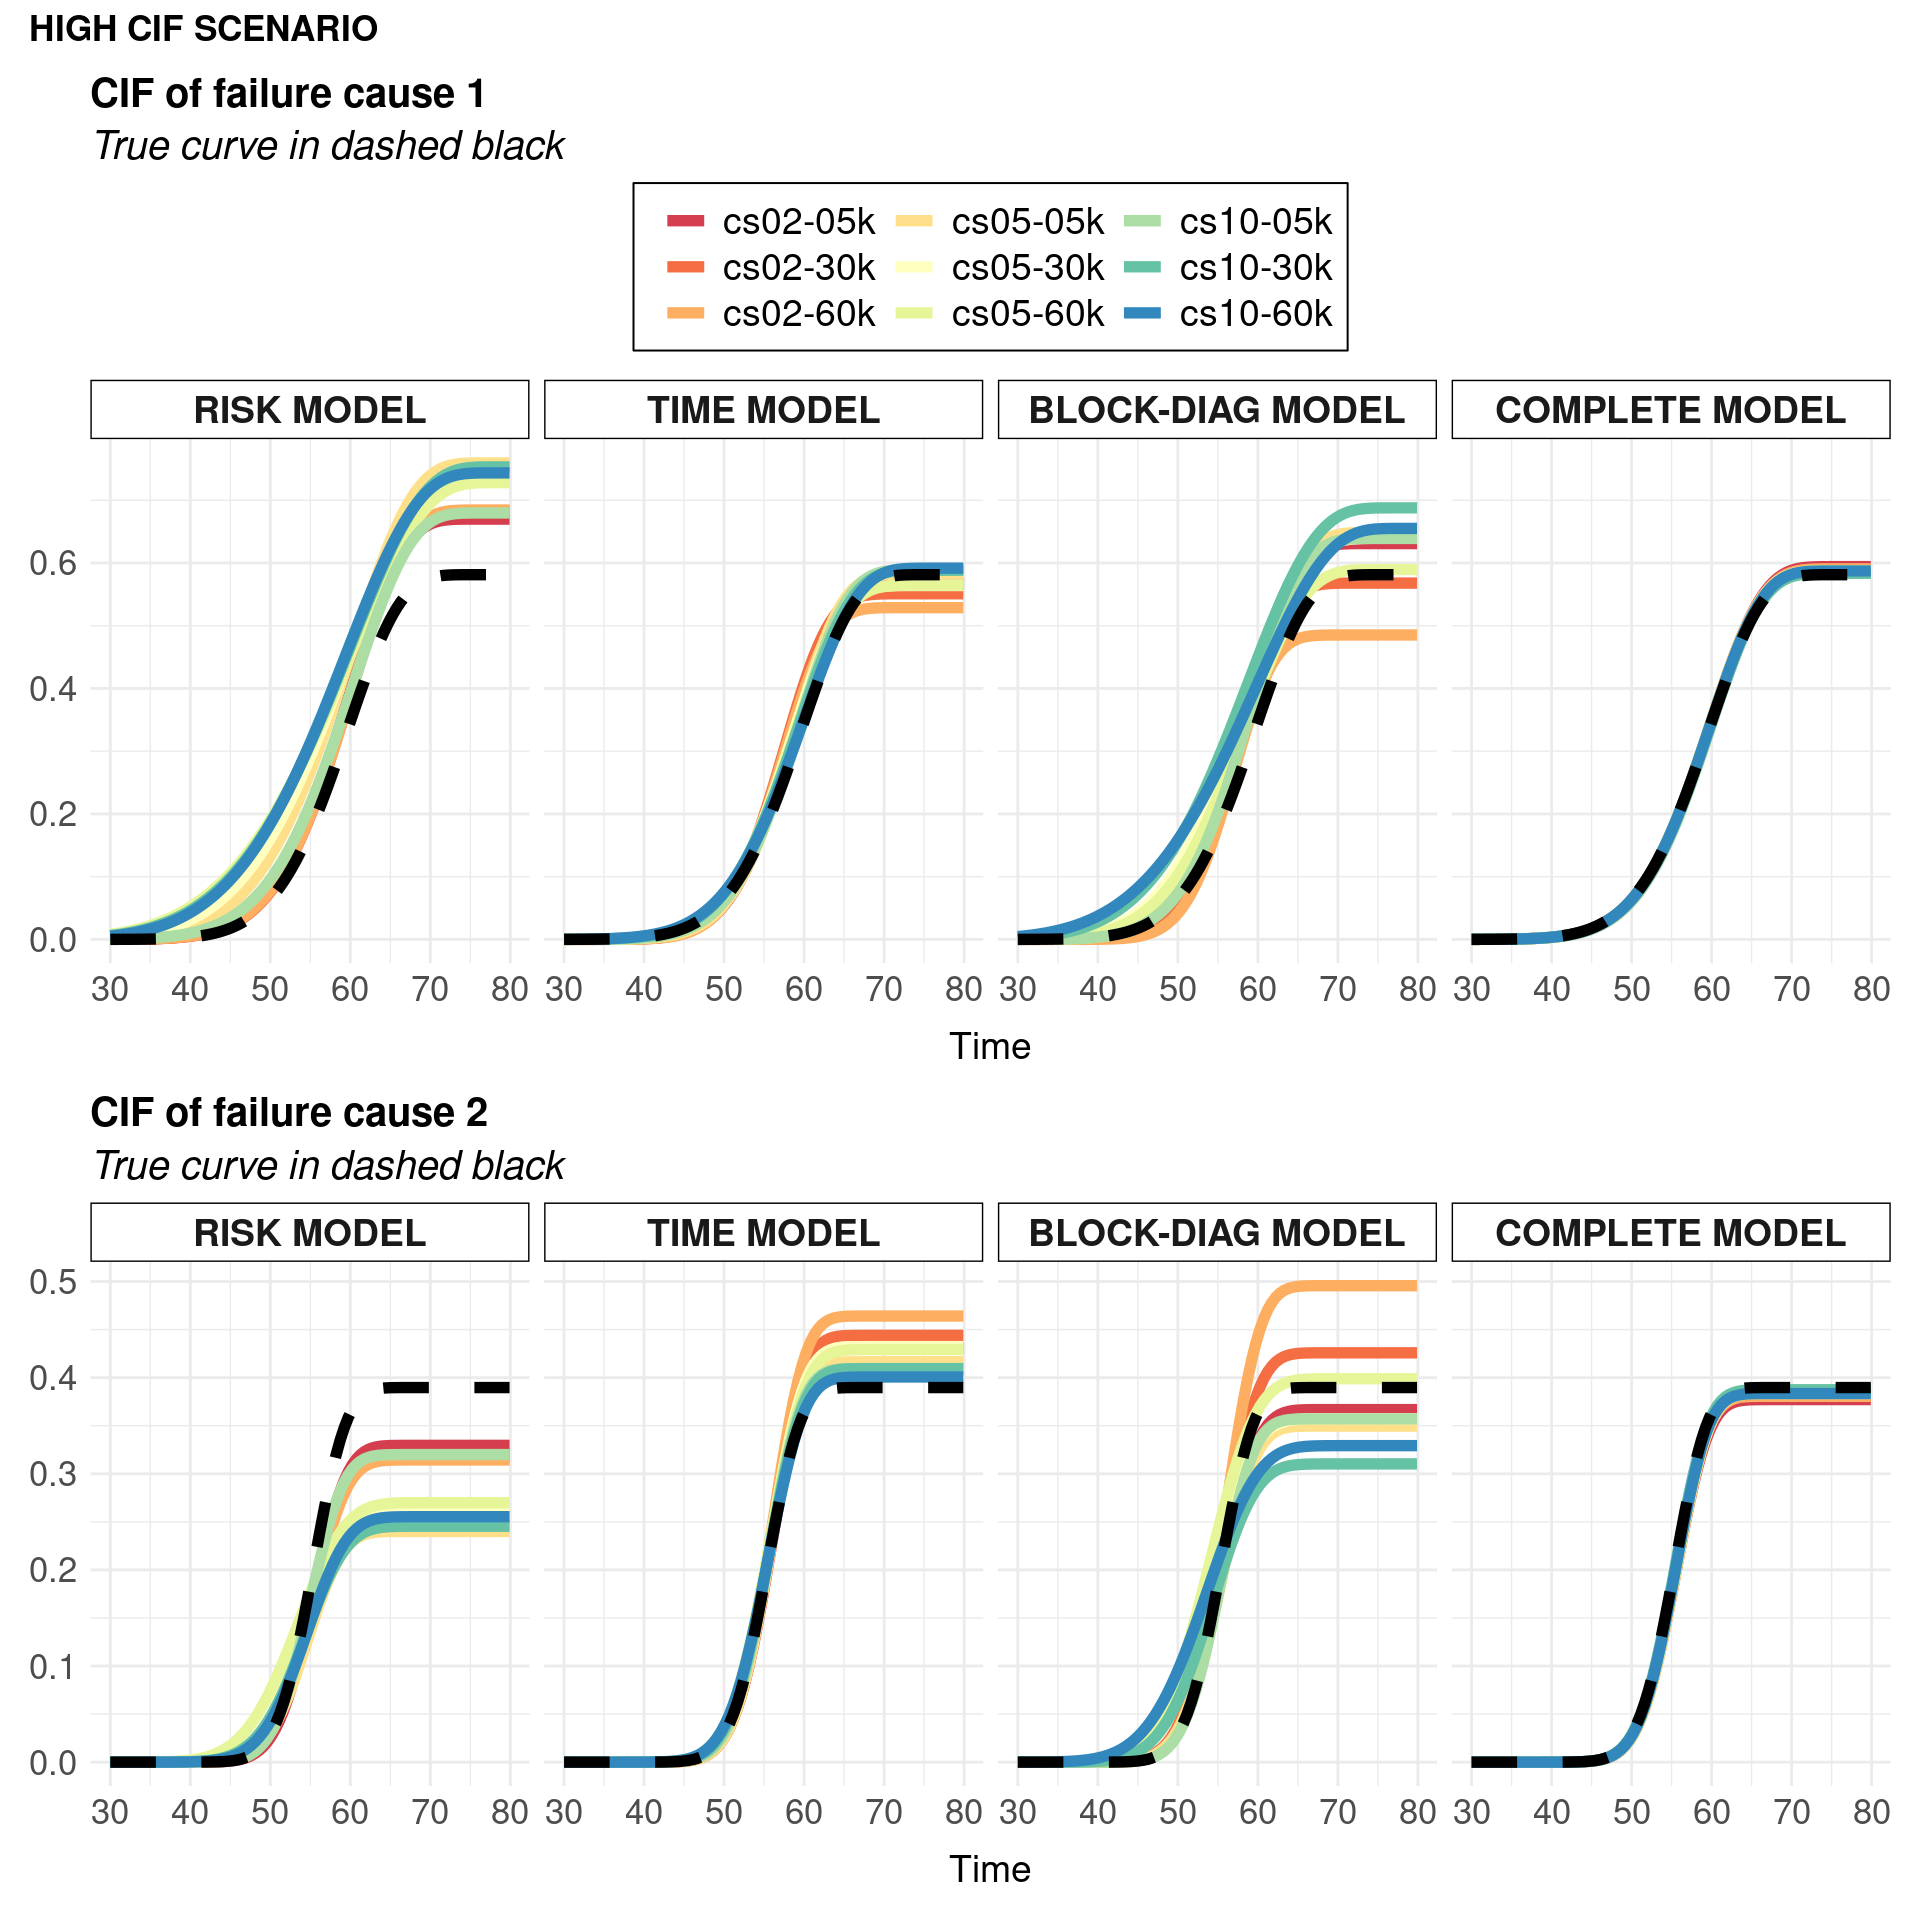
\includegraphics[width=\textwidth]{cifs-1.png}\\
 \begin{footnotesize}
  SOURCE: The author (2021).
 \end{footnotesize}
 \label{fig:cifshigh}
\end{figure}

\begin{figure}[H]
 \setlength{\abovecaptionskip}{.0001pt}
 \caption{LOW CUMULATIVE INCIDENCE FUNCTION (CIF) SCENARIO CURVES}
 \vspace{0.2cm}\centering
 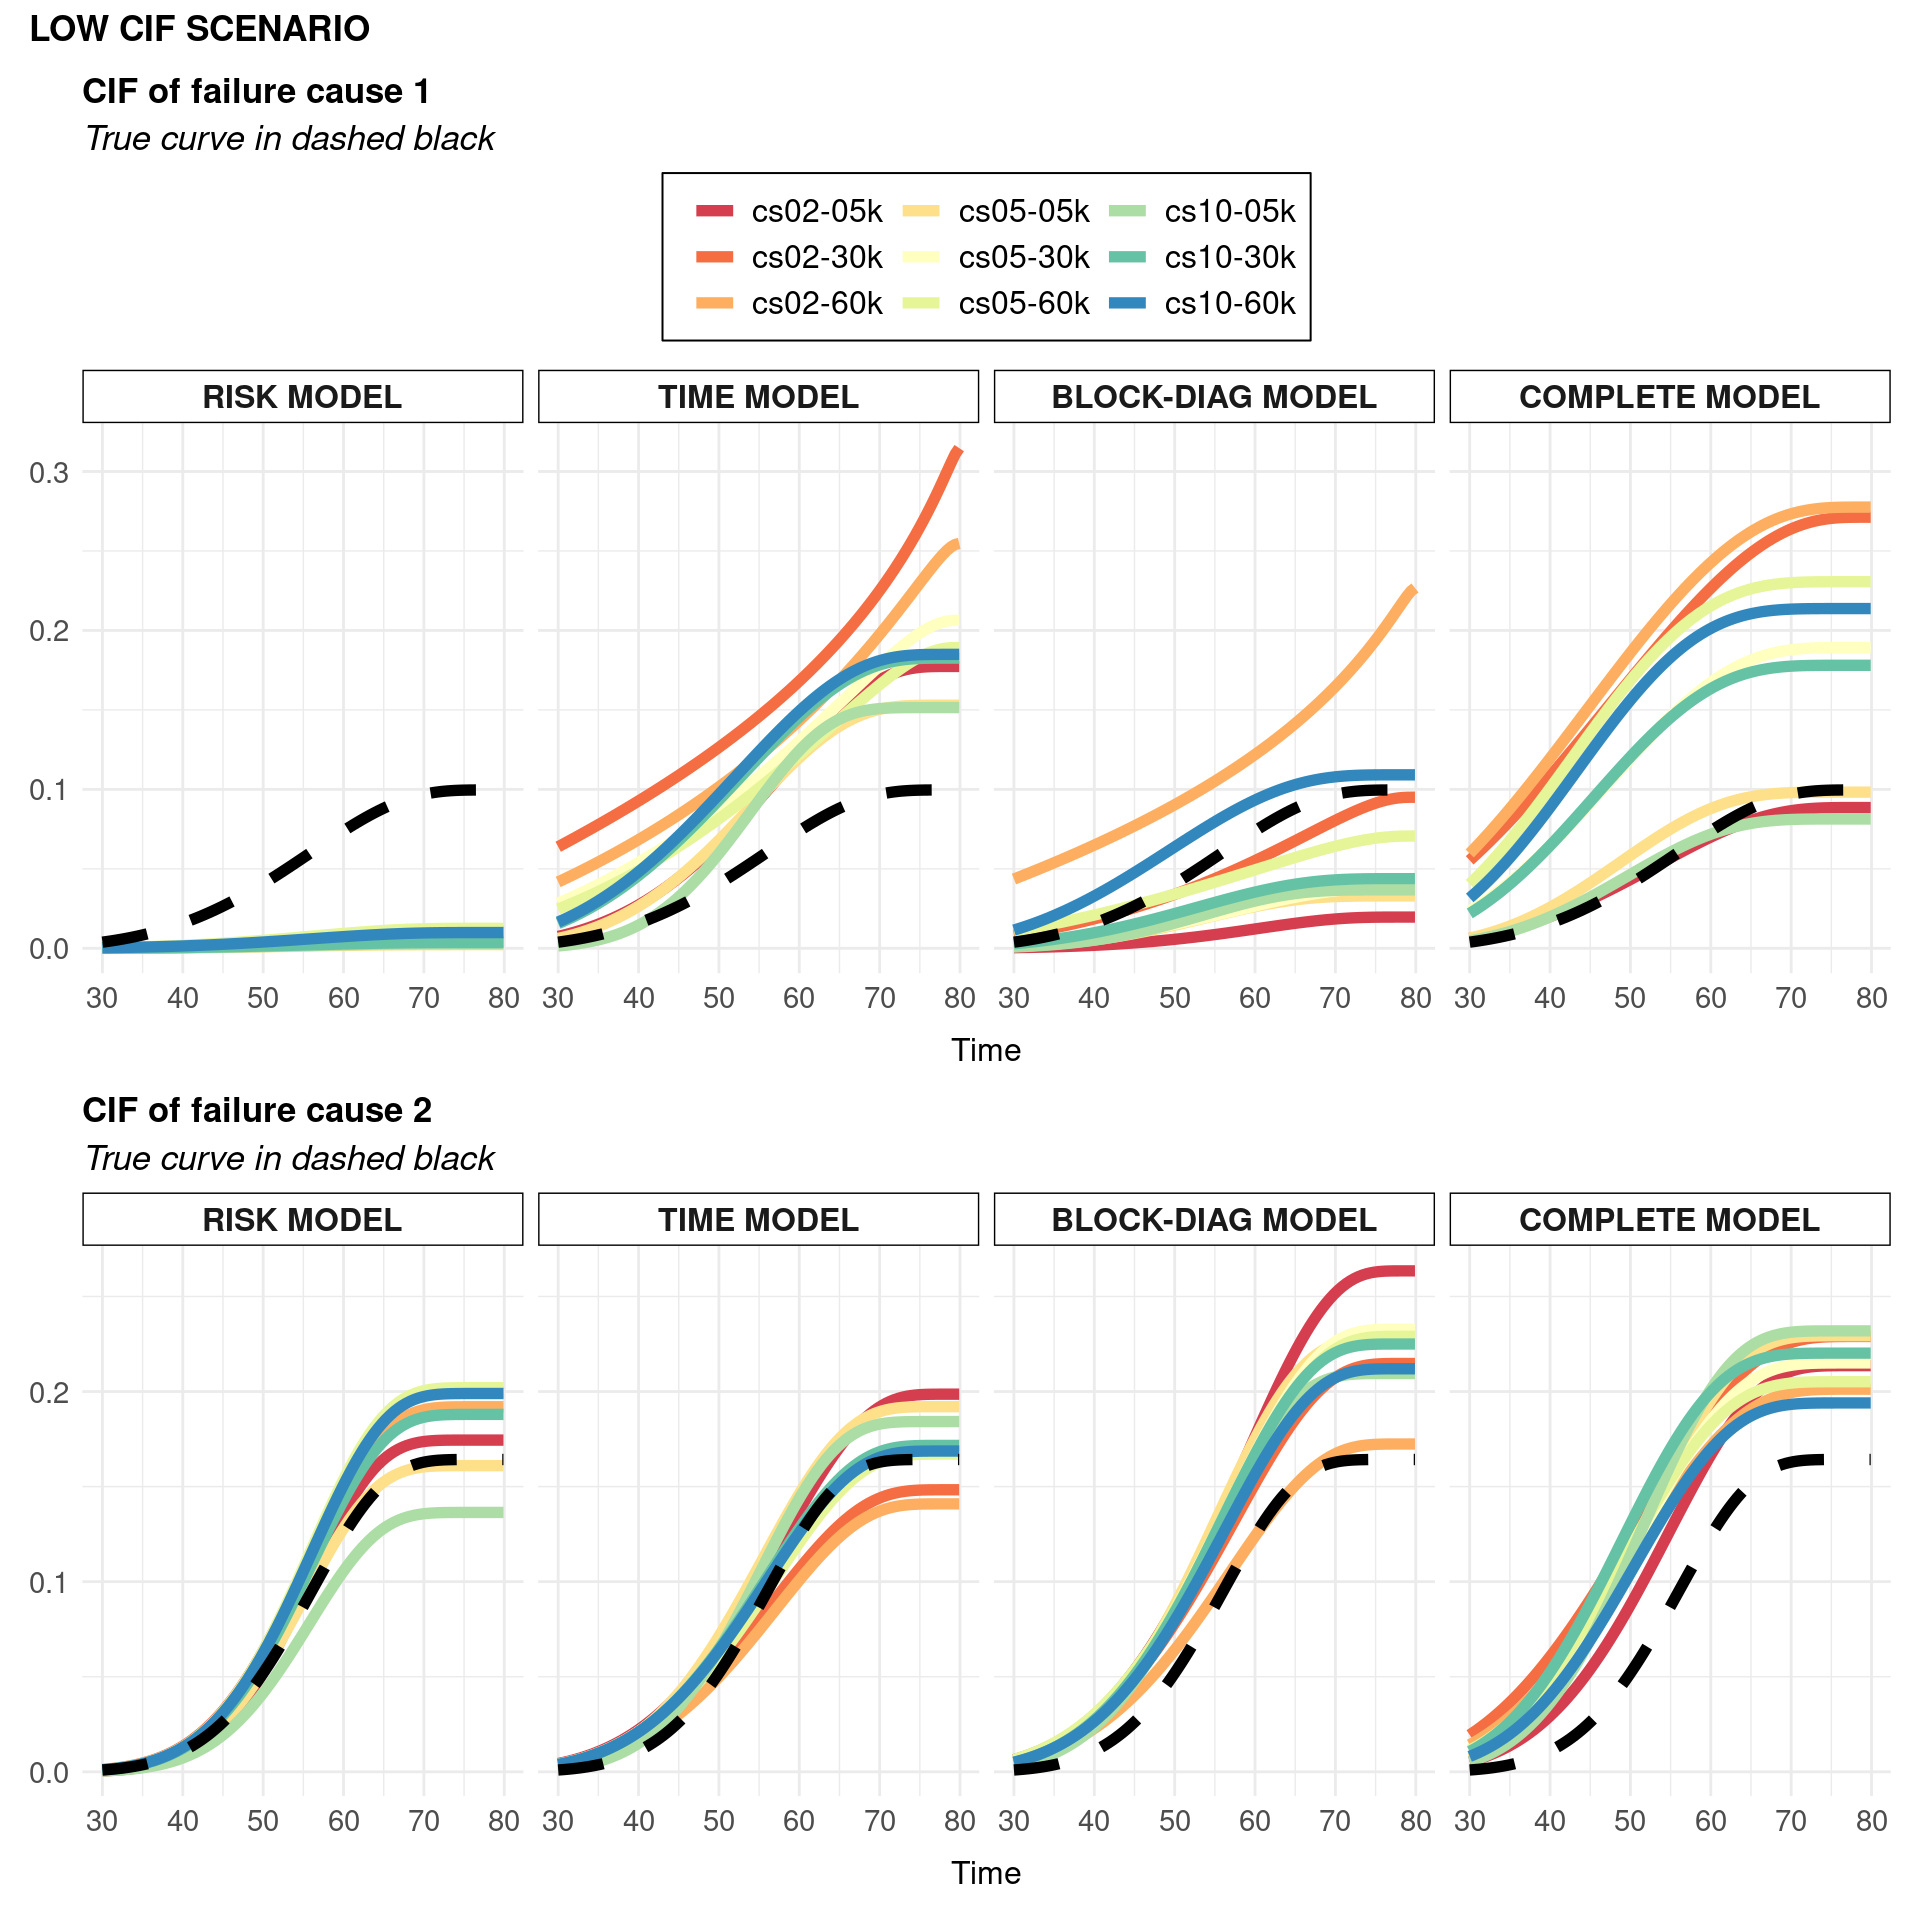
\includegraphics[width=\textwidth]{cifs-2.png}\\
 \begin{footnotesize}
  SOURCE: The author (2021).
 \end{footnotesize}
 \label{fig:cifslow}
\end{figure}

Since in all models we have a latent structure for the within-cluster
dependency, the inherent idea is that this will also affect the
fixed-effect parameter estimates. By taking the average of the
fixed-effect parameter estimates in each of the seventy-two scenarios,
we are able to construct the mean CIF curve for each scenario.

In \autoref{fig:cifshigh} we have all thirty-six curves obtained for the
high CIF scenarios. In dashed black we have the true curve.

%% \begin{figure}[H]
%%  \setlength{\abovecaptionskip}{.0001pt}
%%  \caption{BUILDING \(\Sigma\)}
%%  \vspace{0.2cm}\centering
%%  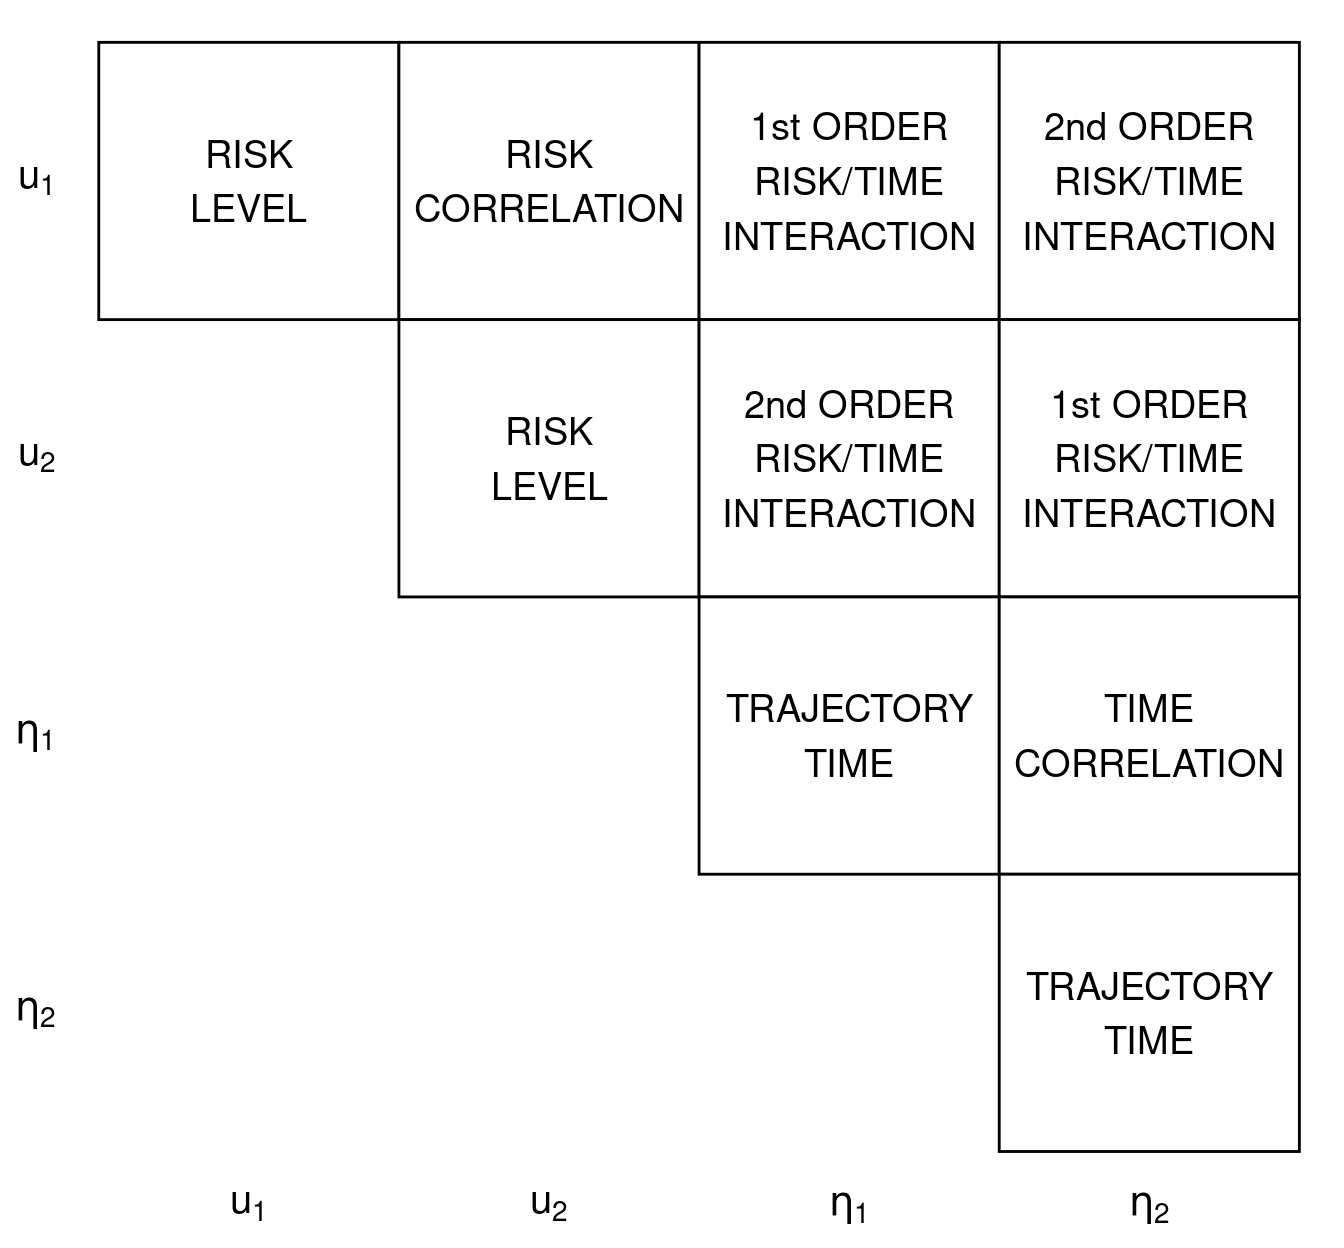
\includegraphics[width=0.75\textwidth]{buildingSigma-1.png}\\
%%  \begin{footnotesize}
%%   SOURCE: The author (2021).
%%  \end{footnotesize}
%%  \label{fig:buildingSigma}
%% \end{figure}

%% \begin{figure}[H]
%%  \setlength{\abovecaptionskip}{.0001pt}
%%  \caption{PARAMETERS CORRELATION}
%%  \vspace{0.2cm}\centering
%%  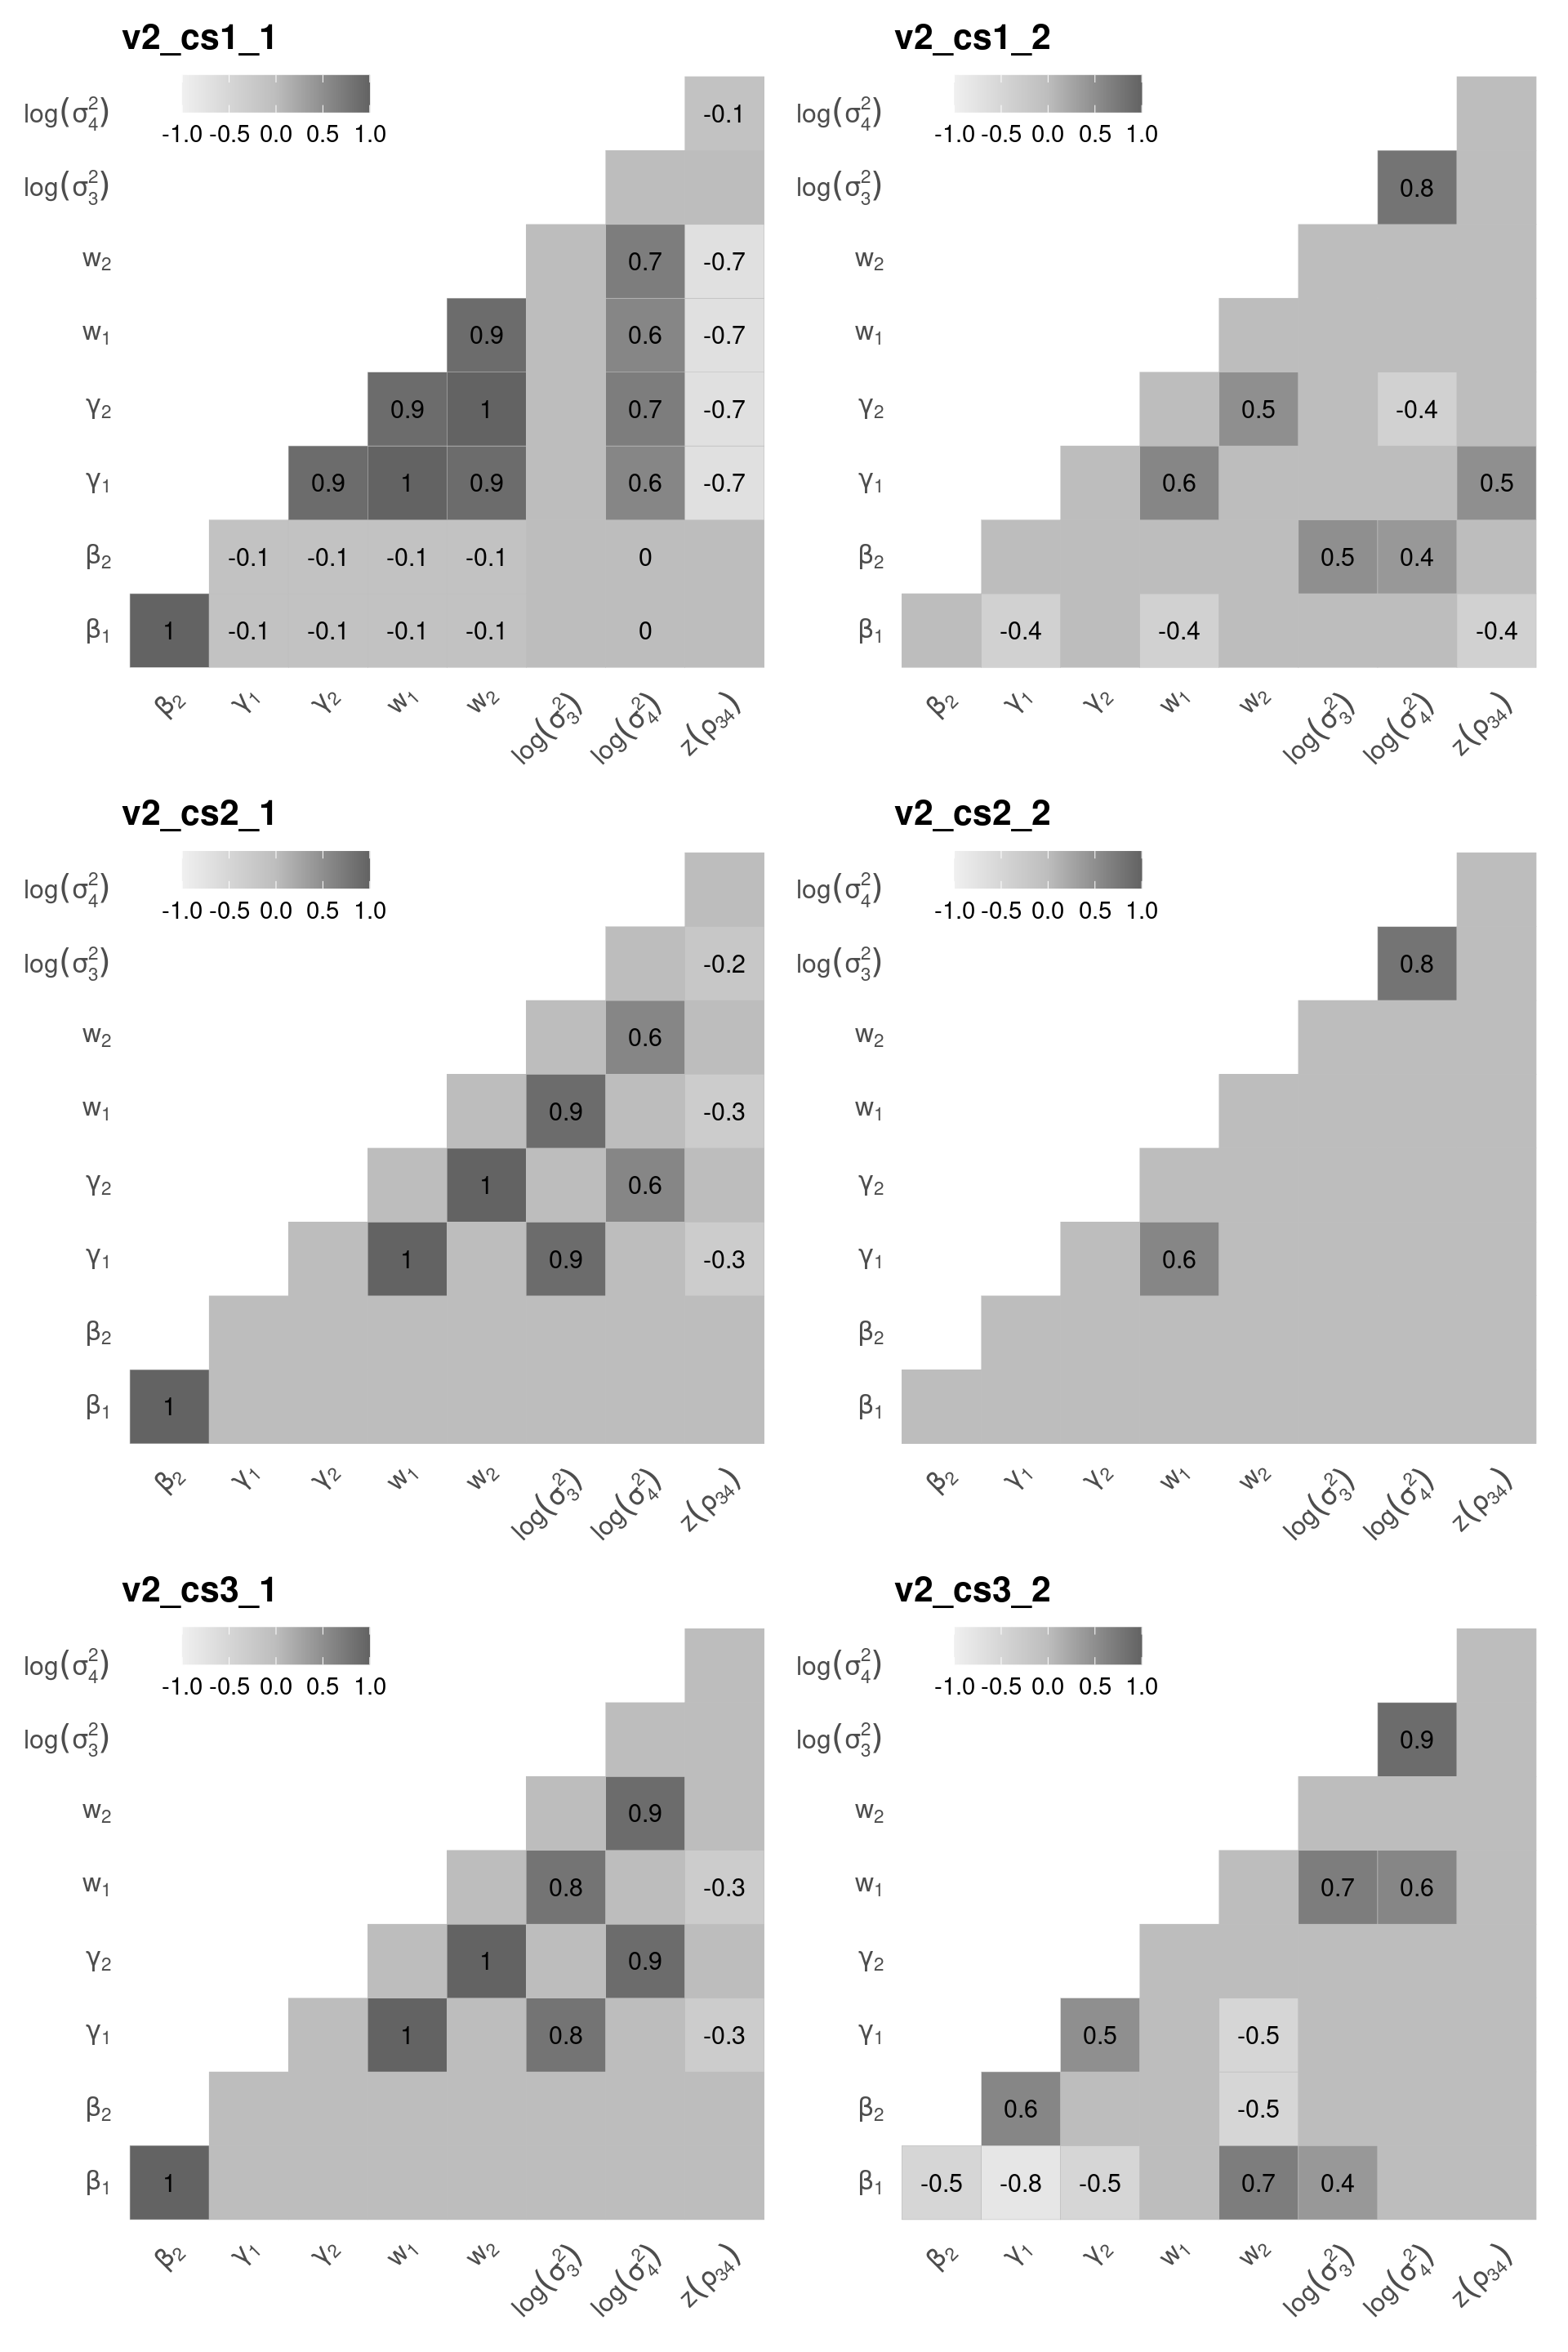
\includegraphics[width=\textwidth]{cor2plot-1.png}\\
%%  \begin{footnotesize}
%%   SOURCE: The author (2021).
%%  \end{footnotesize}
%%  \label{fig:cor2plot}
%% \end{figure}

%% \begin{figure}[H]
%%  \setlength{\abovecaptionskip}{.0001pt}
%%  \caption{VARIANCE-COVARIANCE MATRIX UPPER-TRIANGULAR COMPONENTS}
%%  \vspace{0.2cm}\centering
%%  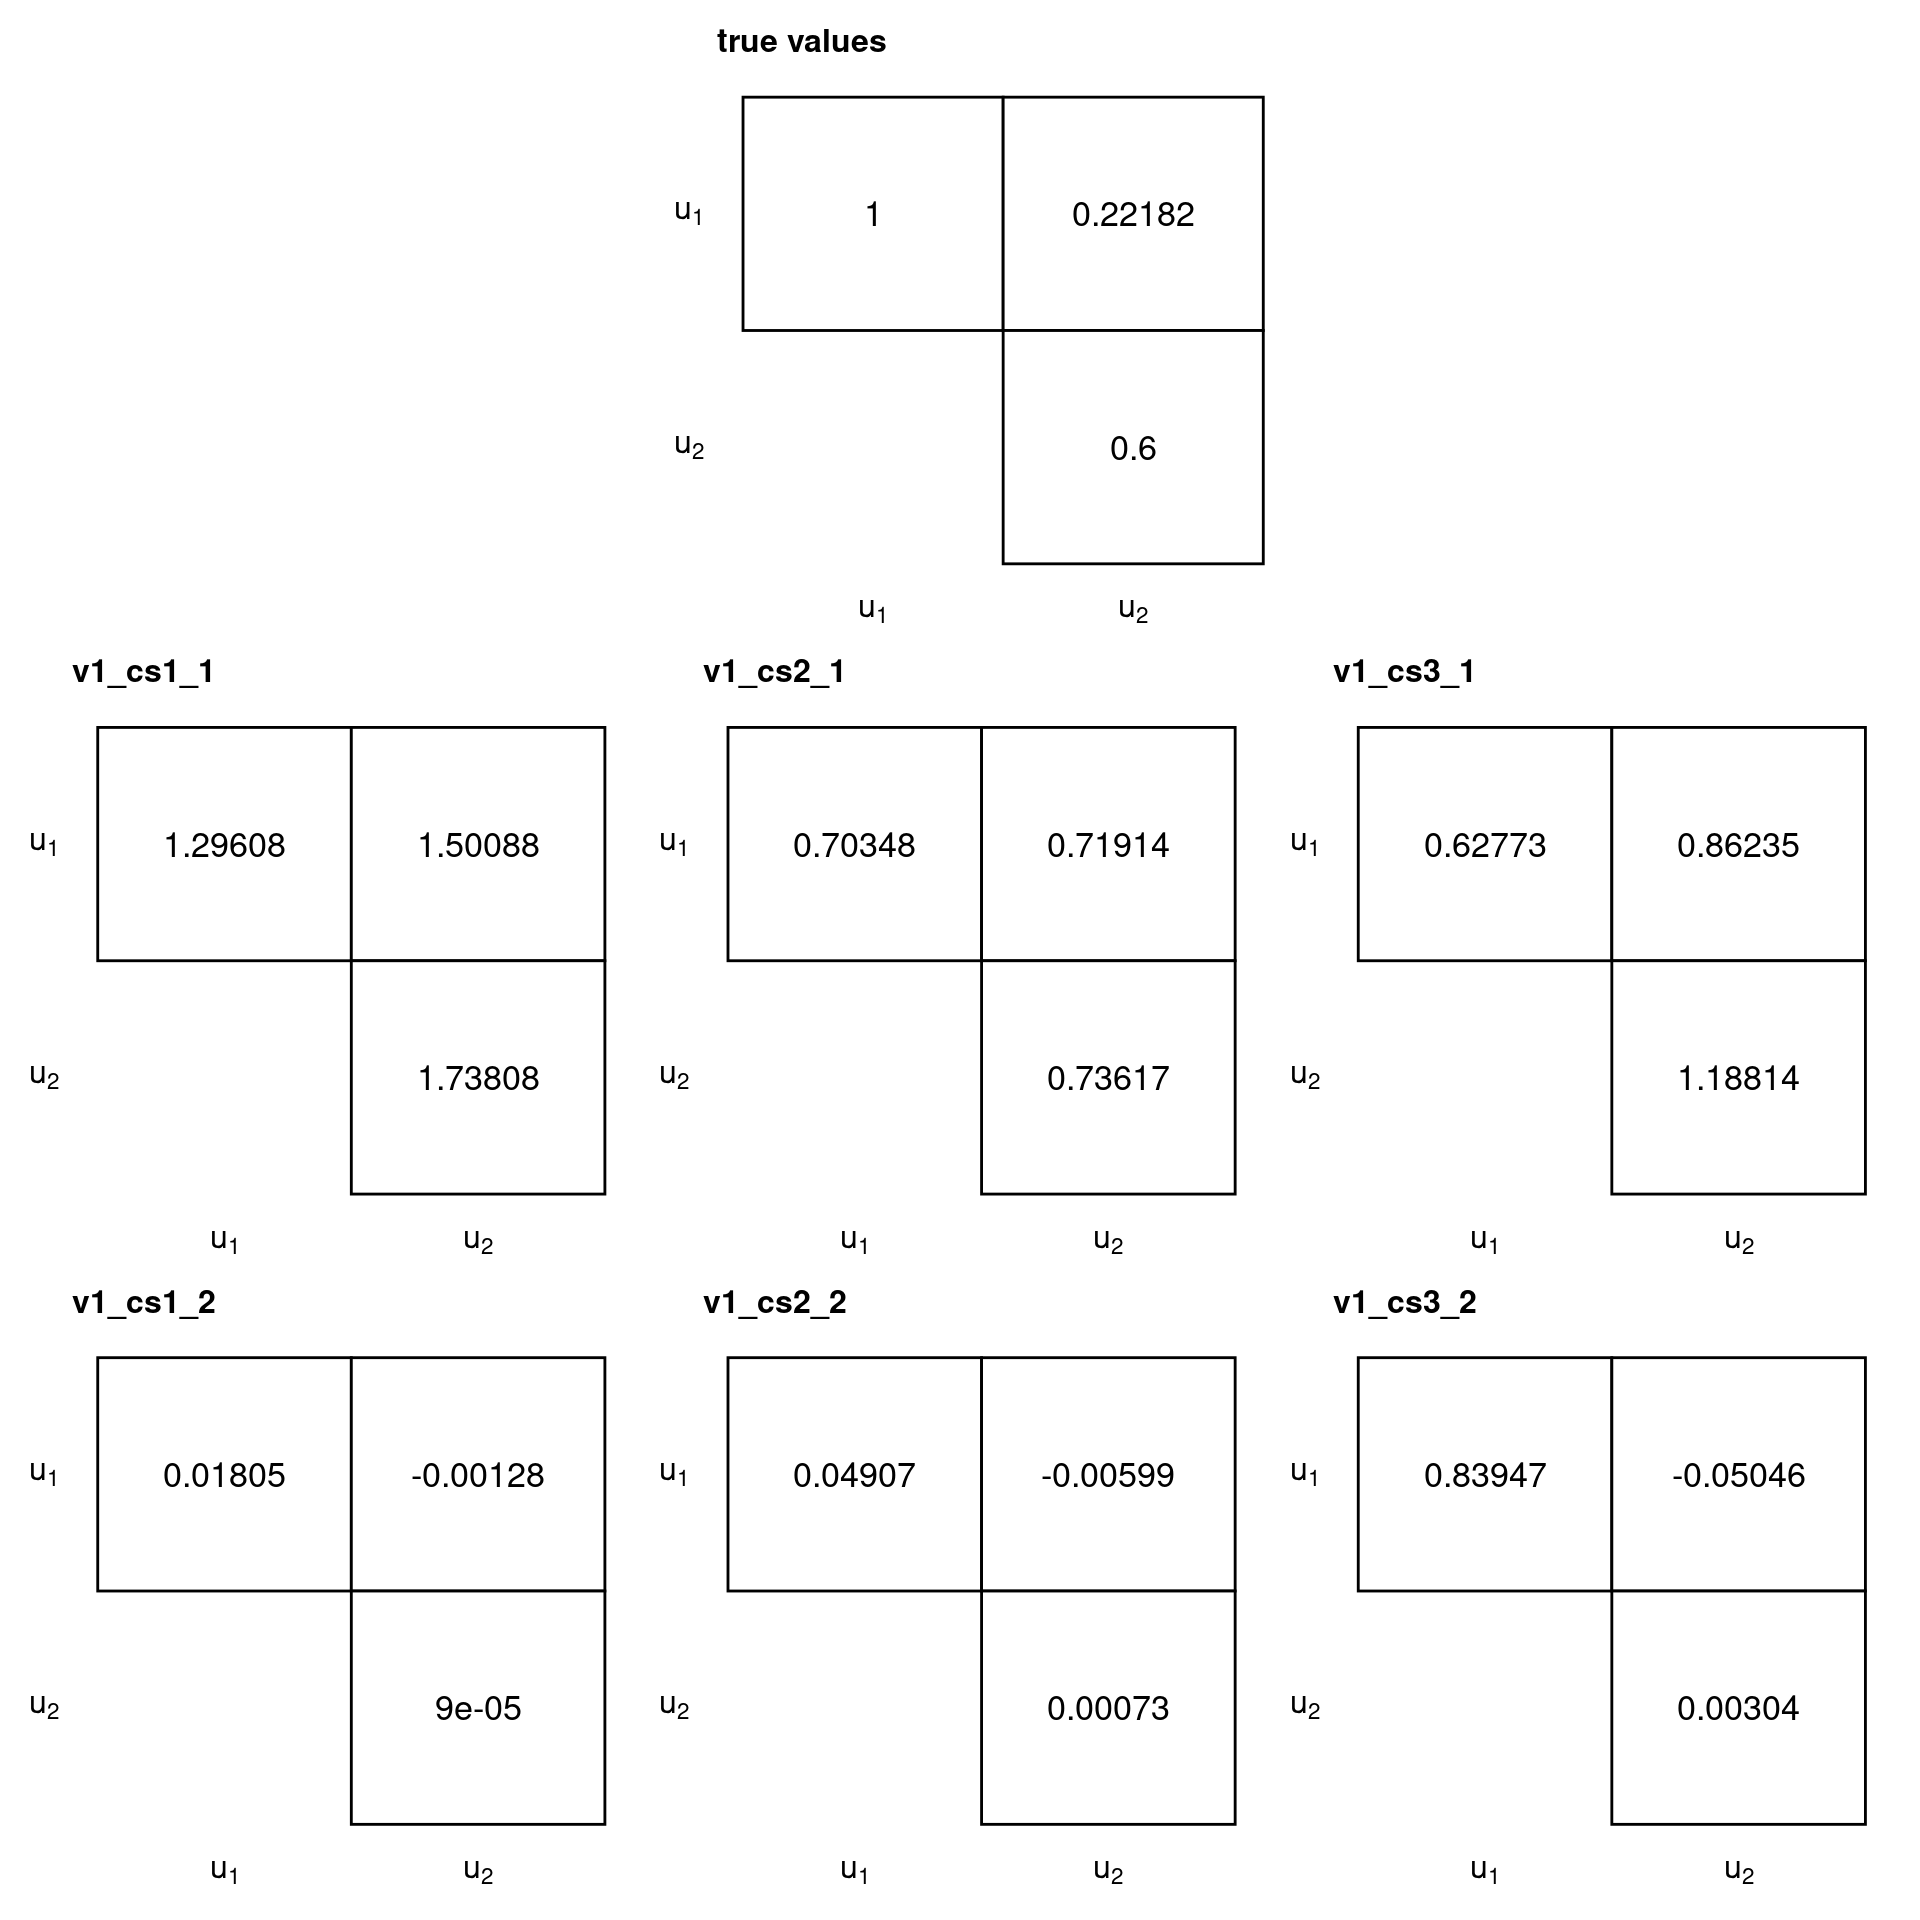
\includegraphics[width=\textwidth]{vcovs-1.png}\\
%%  \begin{footnotesize}
%%   SOURCE: The author (2021).
%%  \end{footnotesize}
%%  \label{fig:vcovs}
%% \end{figure}

% END ==================================================================
